\documentclass{beamer}

% https://ftpmirror1.infania.net/mirror/CTAN/macros/latex/contrib/beamer/doc/beameruserguide.pdf

\usepackage{bibentry}
\usepackage{booktabs}
\usepackage{hyperref}
\usepackage{lmodern}
\usepackage{tikz}
\usepackage{pgf}

\mode<presentation>
\usetheme{default}
\usecolortheme{dove}
\useoutertheme{infolines}

\beamertemplatenavigationsymbolsempty

\setbeamertemplate{bibliography item}{\insertbiblabel}
\setbeamerfont{bibliography item}{size=\scriptsize}
\setbeamerfont{bibliography entry author}{size=\scriptsize}
\setbeamerfont{bibliography entry title}{size=\scriptsize}
\setbeamerfont{bibliography entry location}{size=\scriptsize}
\setbeamerfont{bibliography entry note}{size=\scriptsize}

\title{Learning to Search for Targets}
\subtitle{with Deep Reinforcement Learning}
\author{Oskar Lundin}
\institute{Linköping University}
\date{\today}
\titlegraphic{\includegraphics[scale=0.75]{figures/environments.pdf}}
%\logo{\includegraphics[height=0.5cm]{../report/figures/liu_primary_black_en.pdf}}

\begin{document}

\begin{frame}
    \titlepage
\end{frame}

\begin{frame}
    \frametitle{Outline}
    \tableofcontents
\end{frame}

% should decide on a clear terminology,
% target, distractor, region, view, move, etc.

\chapter{Introduction}
\label{cha:introduction}

% ~3p

In this thesis project, the problem of searching for targets in unknown but familiar environments is addressed.
This chapter presents the motivation behind the project, the research questions that are addressed, and the delimitations. 

\section{Motivation}
\label{sec:motivation}

% This is where the studied problem is described from a general
% point of view and put in a context which makes it clear that
% it is interesting and well worth studying. The aim is to make
% the reader interested in the work and create an urge to
% continue reading.

The ability to visually search for things in an environment is fundamental to intelligent behavior.
We humans are constantly looking for things, be it be it the right book in the bookshelf, a certain keyword in an article or blueberries in the forest.
In many cases, it is important that this search is strategic, efficient, and fast.
Animals need to quickly identify predators, and drivers need to be able to search for pedestrians crossing the road they are driving on.

Automating visual search is of great interest for several reasons.
Visual search is crucial for applications such as search and rescue, surveillance, fire detection, etc.
Autonomous vehicles can both reduce risk and potentially exhibit more intelligent searching behavior than human-controlled ones.

However, while visual search is often seemingly effortless to us humans, it is a complex process.
At the root of the visual search problem is partial observability.
A searcher can only perceive, or pay attention to, a limited region of the searched environment at once.
Therefore which regions to observe and in what order becomes an important decision. 

How humans and animals search for things has been extensively studied in neuroscience~\cite{eckstein_visual_2011,wolfe_visual_2010,nakayama_situating_2011}.
When we search, we use features of the environment to guide our attention~\cite{wolfe_five_2017}.
For example, we know to look for berries at the forest floor, and not to look for boats on land.
Furthermore, search is not purely reactive but involves the use of memory.
We take the history of the search into account in order to select where to move our attention~\cite{wolfe_five_2017}.

Such features can in some cases be quite subtle and difficult to pick up, even for humans.
Manually engineering guidance in accordance with these features can be difficult,
especially if a searching system should be deployed in many different environments.
Doing so manually can be labour intensive, especially if a searching system should be deployed in many different environments.
If one could instead learn the a good searching strategy from a limited set of sample environments this would be circumvented.
Such a system could be taught to search in arbitrary environments without the use of environment-specific rules.

Reinforcement learning~\cite{sutton_reinforcement_2018} is a paradigm that is suited for learning mappings from sensor values to actions.
In recent years, reinforcement learning has been combined with deep learning~\cite{goodfellow_deep_2016} with tremendous success.
It has been used to master arcade games~\cite{mnih_human_2015}, board games~\cite{silver_alphago_2016}, and even complex real-time strategy games~\cite{vinyals_alphastar_2019}.
Several works have also applied reinforcement learning to tasks involving embodied agents with visual input~\cite{minut_mahadevan_2001,mnih_attention_2014,zhu_target_driven_2016,mirowski_navigate_2017}.
This makes it interesting to see if deep reinforcement learning can also be applied to visual search.

\section{Aim}
\label{sec:aim}

The aim of this thesis is to investigate how an intelligent agent that learns to search for targets can be implemented with deep reinforcement learning.
Such an agent should learn the characteristics of the environments it is trained on and utilize this knowledge to effectively search for targets in unseen environments.
We postulate that an effective searcher 

\begin{itemize}
  \item prioritizes regions where the probability of finding a target is high according to previous experience,
  \item is able to search the environment exhaustively,
  \item avoids searching the same area twice unless,
  \item learns how the distribution of targets is correlated to the appearance of the environment,
  \item utilizes information from previously visited regions to decide where to look, and
  \item is able to find multiple targets while minimizing its path length. % test by comparing to optimal travel cost
\end{itemize}

We ask ourselves how an intelligent agent can be trained with reinforcement learning to search with these criteria in mind.
Specifically, we consider scenarios where the agent can only observe a small portion of its environment at any given time through a fixed pan-tilt camera.
The agent has to actively choose where to look in order to gain new information about the environment.
The goal of the agent is to actively locate a set of targets in its environment.

While similar problems have been addressed in the past~\cite{minut_mahadevan_2001}, our impression is that this is the first work to address intelligent search for multiple targets in unseen environments.
Our contributions are as follows:

\begin{itemize}
  %\item We formally introduce the visual search problem for reinforcement learning.
  %\item We discuss the problem from several angles.
  \item We provide a set of environments to evaluate visual search agents.
  \item We propose a method for solving the visual search task with reinforcement learning.
  \item We compare the method to a set of common baseline agents.
  \item We evaluate how well learning agents are able to generalize to unseen environments.
\end{itemize}

\section{Research questions}
\label{sec:research-questions}

% This is where the research questions are described.
% Formulate these as explicit questions, terminated with a
% question mark. A report will usually contain several different
% research questions that are somehow thematically connected.
% There are usually 2-4 questions in total.
% 
% Examples of common types of research questions (simplified
% and generalized):
% 
% \begin{enumerate}
% \item How does technique X affect the possibility of achieving the
%   effect Y?
% 
% \item How can a system (or a solution) for X be realized so
%   that the effect Y is achieved?
% 
% \item What are the alternatives to
%   achieving X, and which alternative gives the best effect considering
%   Y and Z? (This research question is normally broken down in to 2
%   separate questions.)
% 
% \end{enumerate}
% 
% 
% Observe that a very specific research question almost always
% leads to a better thesis report than a general research question
% (it is simply much more difficult to make something good
% from a general research question.)
% 
% The best way to achieve a really good and specific research
% question is to conduct a thorough literature review and get
% familiarized with related research and practice. This leads to
% ideas and terminology which allows one to express oneself
% with precision and also have something valuable to say in the
% discussion chapter. And once a detailed research question
% has been specified, it is much easier to establish a suitable
% method and thus carry out the actual thesis work much faster
% than when starting with a fairly general research question. In
% the end, it usually pays off to spend some extra time in the
% beginning working on the literature review. The thesis
% supervisor can be of assistance in deciding when the research
% question is sufficiently specific and well-grounded in related
% research.

This thesis will address the following questions:

\begin{enumerate}
  \item \label{itm:rq1} How can a learning agent that learns to intelligently search for targets be implemented?
  \item \label{itm:rq2} How does the learning agent compare to random walk, exhaustive search, a human searcher?
  \item \label{itm:rq3} How well does the learning agent generalize to unseen but familiar environments?
\end{enumerate}

\section{Delimitations}
\label{sec:delimitations}

% This is where the main delimitations are described. For
% example, this could be that one has focused the study on a
% specific application domain or target user group. In the
% normal case, the delimitations need not be justified.

This thesis will be focused on the behavioral aspects of the presented problem.
We do not focus on difficult detection problems, but rather strategic actions.
For this reason, targets will deliberately be made easy to detect.
For simplicity, we make the assumption that the searched environment is static.
The appearance of the environment and the location of the targets does not change from one observation to the next.

\section{Theory}

\subsection{Background}

\begin{frame}
    \frametitle{Reinforcement Learning}

    Reinforcement learning (RL) is a paradigm for learning mappings from observations to actions.
    
    Partially observable Markov decision process (POMDP):

    \begin{itemize}
        \item Agent interacts with environment over discrete time steps \(t = 0, 1, 2\dots\)
        \item Takes action \(a_t\) in state \(s_t\)
        \item Perceives observation \(o_t\) 
        \item New state \(s_{t+1}\)
    \end{itemize}

    \begin{figure}
        \centering
        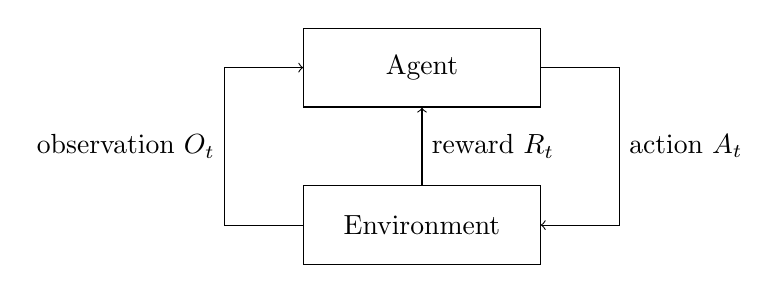
\begin{tikzpicture}[node distance=2cm]
    \tikzstyle{block} = [rectangle,minimum width=3cm,minimum height=1cm,text centered,draw=black,fill=white]
    \node (agent)[block]{Agent};
    \node (environment)[block,below of=agent]{Environment};
    \draw [->] (agent.east) -- ++(1cm,0) -- node [anchor=west]{action \(A_t\)} ++(0,-2cm) -- (environment.east);
    \draw [->] (environment.north) -- node [anchor=west]{reward \(R_t\)} (agent.south);
    \draw [->] (environment.west) -- ++(-1cm,0) -- node [anchor=east]{observation \(O_t\)} ++(0,+2cm) -- (agent.west);
\end{tikzpicture}
    \end{figure}
\end{frame}

\subsection{Related Work}

\begin{frame}
    \frametitle{Search with Reinforcement Learning}

    \dots
\end{frame}
\chapter{Method}
\label{cha:method}

% ~10p

% In this chapter, the method is described in a way which shows how the
% work was actually carried out. The description must be precise and
% well thought through. Consider the scientific term
% replicability. Replicability means that someone reading a scientific
% report should be able to follow the method description and then carry
% out the same study and check whether the results obtained are
% similar. Achieving replicability is not always relevant, but precision
% and clarity is.
% 
% Sometimes the work is separated into different parts, e.g.  pre-study,
% implementation and evaluation. In such cases it is recommended that
% the method chapter is structured accordingly with suitable named
% sub-headings.

In this chapter, the method used is described.
Section \ref{sec:problem} formalizes the problem solved.
Section \ref{sec:environment} details the environment used to evaluate solutions.
Section \ref{sec:baseline} describes the baseline learning method.
Section \ref{sec:approach} describes the approach used to solve the problem with a learning agent.
Section \ref{sec:experiments} describes the experiments conducted to answer research questions \ref{itm:rq2} and \ref{itm:rq3}.

\section{Problem Statement}
\label{sec:problem}

% Maybe keep the POMDP stuff in environment section

We can now formally define the problem of searching for targets in unknown environments.

We denote the task by \(\langle \mathcal{M}, \mathcal{T}_0 \rangle\), where \(\mathcal{M}\) is a POMDP and \(\mathcal{T}_0\) is the probability distribution on the initial states.
The state is defined by a (Euclidean) space \(S \subset \mathbb{R}^d\) which we refer to as the \textit{scene}.
At each timestep, the agent observes a subspace \(V \subset S\) of the environment which we refer to as the \textit{view}.
The actions in \(\mathcal{A}\) transform the view.
In the scene, there is a set of \(N\) targets \(T = \{t_0, t_1, \dots t_N | t_i \in S\}\).
With a final trigger action, the agent can indicate that there is one or more target in the view.
The goal of the agent is to select actions that bring each target into view and indicate that they are visible with the trigger action, while minimizing the number of actions taken.
The observations \(o \in \Omega\) are tuples \(o = \left\langle x, p \right\rangle\),
where \(x \in \mathbb{R}^{3 \times W \times H}\) is an RGB image representing the current view, and \(p \in S\) is the position of the agent.
If \(T \cap V \neq \varnothing\) there are \(h = \left\lvert T \cap V \right\rvert\) targets in view.

\section{Environments}
\label{sec:environments}

To train an test an agent for the problem, we use three different environments.
The three environments have different characteristics to test the applicability of the evaluated approaches.
In each environment there is a scene with a background of distractors and a foreground of targets.
The scenes are drawn from some unknown distribution.
The background and foreground are assumed to be correlated.
This means that by looking at the background, an agent should sometimes be able to deduce a suitable action.

For the position, we assume the presense of some oracle.
In many realistic scenarios this is the case (GPS, pan/tilt, etc.).
If how each action moves the agent is well-defined, we do not need the position at all.
We can use relative positions instead of absolute ones.
Some of the baselines do not use the position.

The action space is the same in all environments:

\[
    \mathcal{A} = \lbrace \mathtt{UP}, \mathtt{DOWN}, \mathtt{LEFT}, \mathtt{RIGHT}, \mathtt{TRIGGER} \rbrace,
\]

\(\mathtt{UP}\), \(\mathtt{DOWN}\), \(\mathtt{LEFT}\), and \(\mathtt{RIGHT}\) translate the view and \(\mathtt{TRIGGER}\) indicates that a target is in view.
% rotates in third environment though

We experiment with three rewards signals.
The first reward signal is defined as

\[
    \mathcal{R}(s_t, a_t) =
    \begin{cases}
        10h & \text{if \(a_t = \mathtt{TRIGGER}\) and a target is in view,} \\
        -1  & \text{otherwise.}
    \end{cases}
\]

with \(h = \left\lvert T \cap V \right\rvert\). 
We argue that this reward provides a suitable inductive bias for the task at hand.
Early experiments show that a constant reward of \(r_t = -1\) that simply incentivizes the agent to complete the episode as quickly as possible converge too slowly for large state spaces.
The reward for finding a target speeds up training without deviating from the goal of the task -
targets should be triggered when in view, but triggers when targets are out of view should be penalized.
The constant penalty of \(-1\) in all other cases assures that the agent is rewarded for quick episode completion.

In practice, early experiments show that even this reward might be too sparse.
To speed up training, we experiment with two extensions to the reward:

\[
    \mathcal{R}'(s_t, a_t) =
    \begin{cases}
        1 & \text{if \(a_t \neq \mathtt{TRIGGER}\) moves the view closer to the nearest target, and} \\
        \mathcal{R}(s_t, a_t) & \text{otherwise}.
    \end{cases}
\]

\[
    \mathcal{R}''(s_t, a_t) =
    \begin{cases}
        1 & \text{if \(a_t \neq \mathtt{TRIGGER}\) moves the view to a previously unseen subspace, and} \\
        \mathcal{R}(s_t, a_t) & \text{otherwise}.
    \end{cases}
\]


These three reward signals are interesting to compare for a few reasons.
\(R\) does not clearly mediate to the agent what actions are desireable until a target is found.
It may therefore lead to slow learning, but it also does not steer away from the goal of finding targets quickly.
\(R'\) uses the supervised distance between targets and the agents, which is available during training.
This is similar to the reward used by \cite{caicedo_active_2015} and \cite{ghesu_multi_scale_2019}.
In addition to speeding up learning, we hypothesize that this reward may help the agent pick up correlations between scene appearance and target probability.
However, it can never yield policies that search exhaustively as such actions are never rewarded.
It may therefore perform worse during testing where the reward is not available to the agent.
It will also not learn to take the shortest paths in the general case, as selecting waypoints greedily does not yield optimal paths.
\(R''\) strikes a balance between the two other signals by instead incentivizing exploration.
This should cause the agent to learn to search the environment exhaustively.
% tabu search
% optimal paths

The episode is terminated when all targets have been found, or when 1000 time steps have passed.
Terminating episodes early this way is common to speed up training~\cite{pardo_timelimits_2022}.

% Averaged over all possible samples, the probability of targets should be uniform over the scene.
% to make comparison with exhaustive search fair
% I think?

\subsection{Gaussian Environment}
% environment 1: easy, understandable

The first environment is the simplest environment. 
The scene is described by a 256x256 RGB image.
The agent observes a 64x64 sub-image at each time step.
In the image there are three Gaussian kernels with random positions.
The height of the kernel is indicated by a higher intensity in the blue channel.
Targets are 1x1 pixels in the red channel.
The locations of the targets are randomized weighted by the height of the Gaussian kernels.
This means that the more intense the blue channel, the higher the probability of a target.
The idea with this environment is to test that the method learns what we want it to learn.
There is a clear correlation between observations and desirable actions.
It is also easy to determine whether the agent acts well in this environment.
Our feeling is that this is something that previous similar works has not done. % cite

\begin{figure}
    \centering
    %% Creator: Matplotlib, PGF backend
%%
%% To include the figure in your LaTeX document, write
%%   \input{<filename>.pgf}
%%
%% Make sure the required packages are loaded in your preamble
%%   \usepackage{pgf}
%%
%% Also ensure that all the required font packages are loaded; for instance,
%% the lmodern package is sometimes necessary when using math font.
%%   \usepackage{lmodern}
%%
%% Figures using additional raster images can only be included by \input if
%% they are in the same directory as the main LaTeX file. For loading figures
%% from other directories you can use the `import` package
%%   \usepackage{import}
%%
%% and then include the figures with
%%   \import{<path to file>}{<filename>.pgf}
%%
%% Matplotlib used the following preamble
%%   \usepackage{fontspec}
%%   \setmainfont{DejaVuSerif.ttf}[Path=\detokenize{/home/oslund/.local/lib/python3.8/site-packages/matplotlib/mpl-data/fonts/ttf/}]
%%   \setsansfont{DejaVuSans.ttf}[Path=\detokenize{/home/oslund/.local/lib/python3.8/site-packages/matplotlib/mpl-data/fonts/ttf/}]
%%   \setmonofont{DejaVuSansMono.ttf}[Path=\detokenize{/home/oslund/.local/lib/python3.8/site-packages/matplotlib/mpl-data/fonts/ttf/}]
%%
\begingroup%
\makeatletter%
\begin{pgfpicture}%
\pgfpathrectangle{\pgfpointorigin}{\pgfqpoint{4.777896in}{3.713045in}}%
\pgfusepath{use as bounding box, clip}%
\begin{pgfscope}%
\pgfsetbuttcap%
\pgfsetmiterjoin%
\definecolor{currentfill}{rgb}{1.000000,1.000000,1.000000}%
\pgfsetfillcolor{currentfill}%
\pgfsetlinewidth{0.000000pt}%
\definecolor{currentstroke}{rgb}{1.000000,1.000000,1.000000}%
\pgfsetstrokecolor{currentstroke}%
\pgfsetdash{}{0pt}%
\pgfpathmoveto{\pgfqpoint{0.000000in}{0.000000in}}%
\pgfpathlineto{\pgfqpoint{4.777896in}{0.000000in}}%
\pgfpathlineto{\pgfqpoint{4.777896in}{3.713045in}}%
\pgfpathlineto{\pgfqpoint{0.000000in}{3.713045in}}%
\pgfpathlineto{\pgfqpoint{0.000000in}{0.000000in}}%
\pgfpathclose%
\pgfusepath{fill}%
\end{pgfscope}%
\begin{pgfscope}%
\pgfsetbuttcap%
\pgfsetmiterjoin%
\definecolor{currentfill}{rgb}{1.000000,1.000000,1.000000}%
\pgfsetfillcolor{currentfill}%
\pgfsetlinewidth{0.000000pt}%
\definecolor{currentstroke}{rgb}{0.000000,0.000000,0.000000}%
\pgfsetstrokecolor{currentstroke}%
\pgfsetstrokeopacity{0.000000}%
\pgfsetdash{}{0pt}%
\pgfpathmoveto{\pgfqpoint{0.302637in}{0.339475in}}%
\pgfpathlineto{\pgfqpoint{3.536524in}{0.339475in}}%
\pgfpathlineto{\pgfqpoint{3.536524in}{3.573362in}}%
\pgfpathlineto{\pgfqpoint{0.302637in}{3.573362in}}%
\pgfpathlineto{\pgfqpoint{0.302637in}{0.339475in}}%
\pgfpathclose%
\pgfusepath{fill}%
\end{pgfscope}%
\begin{pgfscope}%
\pgfpathrectangle{\pgfqpoint{0.302637in}{0.339475in}}{\pgfqpoint{3.233887in}{3.233887in}}%
\pgfusepath{clip}%
\pgfsys@transformshift{0.302637in}{0.339475in}%
\pgftext[left,bottom]{\includegraphics[interpolate=true,width=3.236667in,height=3.236667in]{gaussian-img0.png}}%
\end{pgfscope}%
\begin{pgfscope}%
\pgfpathrectangle{\pgfqpoint{0.302637in}{0.339475in}}{\pgfqpoint{3.233887in}{3.233887in}}%
\pgfusepath{clip}%
\pgfsetbuttcap%
\pgfsetroundjoin%
\pgfsetlinewidth{0.250937pt}%
\definecolor{currentstroke}{rgb}{0.000000,0.000000,0.000000}%
\pgfsetstrokecolor{currentstroke}%
\pgfsetdash{{0.925000pt}{0.400000pt}}{0.000000pt}%
\pgfpathmoveto{\pgfqpoint{0.305163in}{0.339475in}}%
\pgfpathlineto{\pgfqpoint{0.305163in}{3.573362in}}%
\pgfusepath{stroke}%
\end{pgfscope}%
\begin{pgfscope}%
\pgfsetbuttcap%
\pgfsetroundjoin%
\definecolor{currentfill}{rgb}{0.150000,0.150000,0.150000}%
\pgfsetfillcolor{currentfill}%
\pgfsetlinewidth{1.254687pt}%
\definecolor{currentstroke}{rgb}{0.150000,0.150000,0.150000}%
\pgfsetstrokecolor{currentstroke}%
\pgfsetdash{}{0pt}%
\pgfsys@defobject{currentmarker}{\pgfqpoint{0.000000in}{-0.083333in}}{\pgfqpoint{0.000000in}{0.000000in}}{%
\pgfpathmoveto{\pgfqpoint{0.000000in}{0.000000in}}%
\pgfpathlineto{\pgfqpoint{0.000000in}{-0.083333in}}%
\pgfusepath{stroke,fill}%
}%
\begin{pgfscope}%
\pgfsys@transformshift{0.305163in}{0.339475in}%
\pgfsys@useobject{currentmarker}{}%
\end{pgfscope}%
\end{pgfscope}%
\begin{pgfscope}%
\definecolor{textcolor}{rgb}{0.150000,0.150000,0.150000}%
\pgfsetstrokecolor{textcolor}%
\pgfsetfillcolor{textcolor}%
\pgftext[x=0.305163in,y=0.207530in,,top]{\color{textcolor}\rmfamily\fontsize{8.000000}{9.600000}\selectfont 0}%
\end{pgfscope}%
\begin{pgfscope}%
\pgfpathrectangle{\pgfqpoint{0.302637in}{0.339475in}}{\pgfqpoint{3.233887in}{3.233887in}}%
\pgfusepath{clip}%
\pgfsetbuttcap%
\pgfsetroundjoin%
\pgfsetlinewidth{0.250937pt}%
\definecolor{currentstroke}{rgb}{0.000000,0.000000,0.000000}%
\pgfsetstrokecolor{currentstroke}%
\pgfsetdash{{0.925000pt}{0.400000pt}}{0.000000pt}%
\pgfpathmoveto{\pgfqpoint{0.628552in}{0.339475in}}%
\pgfpathlineto{\pgfqpoint{0.628552in}{3.573362in}}%
\pgfusepath{stroke}%
\end{pgfscope}%
\begin{pgfscope}%
\pgfsetbuttcap%
\pgfsetroundjoin%
\definecolor{currentfill}{rgb}{0.150000,0.150000,0.150000}%
\pgfsetfillcolor{currentfill}%
\pgfsetlinewidth{1.254687pt}%
\definecolor{currentstroke}{rgb}{0.150000,0.150000,0.150000}%
\pgfsetstrokecolor{currentstroke}%
\pgfsetdash{}{0pt}%
\pgfsys@defobject{currentmarker}{\pgfqpoint{0.000000in}{-0.083333in}}{\pgfqpoint{0.000000in}{0.000000in}}{%
\pgfpathmoveto{\pgfqpoint{0.000000in}{0.000000in}}%
\pgfpathlineto{\pgfqpoint{0.000000in}{-0.083333in}}%
\pgfusepath{stroke,fill}%
}%
\begin{pgfscope}%
\pgfsys@transformshift{0.628552in}{0.339475in}%
\pgfsys@useobject{currentmarker}{}%
\end{pgfscope}%
\end{pgfscope}%
\begin{pgfscope}%
\definecolor{textcolor}{rgb}{0.150000,0.150000,0.150000}%
\pgfsetstrokecolor{textcolor}%
\pgfsetfillcolor{textcolor}%
\pgftext[x=0.628552in,y=0.207530in,,top]{\color{textcolor}\rmfamily\fontsize{8.000000}{9.600000}\selectfont 1}%
\end{pgfscope}%
\begin{pgfscope}%
\pgfpathrectangle{\pgfqpoint{0.302637in}{0.339475in}}{\pgfqpoint{3.233887in}{3.233887in}}%
\pgfusepath{clip}%
\pgfsetbuttcap%
\pgfsetroundjoin%
\pgfsetlinewidth{0.250937pt}%
\definecolor{currentstroke}{rgb}{0.000000,0.000000,0.000000}%
\pgfsetstrokecolor{currentstroke}%
\pgfsetdash{{0.925000pt}{0.400000pt}}{0.000000pt}%
\pgfpathmoveto{\pgfqpoint{0.951941in}{0.339475in}}%
\pgfpathlineto{\pgfqpoint{0.951941in}{3.573362in}}%
\pgfusepath{stroke}%
\end{pgfscope}%
\begin{pgfscope}%
\pgfsetbuttcap%
\pgfsetroundjoin%
\definecolor{currentfill}{rgb}{0.150000,0.150000,0.150000}%
\pgfsetfillcolor{currentfill}%
\pgfsetlinewidth{1.254687pt}%
\definecolor{currentstroke}{rgb}{0.150000,0.150000,0.150000}%
\pgfsetstrokecolor{currentstroke}%
\pgfsetdash{}{0pt}%
\pgfsys@defobject{currentmarker}{\pgfqpoint{0.000000in}{-0.083333in}}{\pgfqpoint{0.000000in}{0.000000in}}{%
\pgfpathmoveto{\pgfqpoint{0.000000in}{0.000000in}}%
\pgfpathlineto{\pgfqpoint{0.000000in}{-0.083333in}}%
\pgfusepath{stroke,fill}%
}%
\begin{pgfscope}%
\pgfsys@transformshift{0.951941in}{0.339475in}%
\pgfsys@useobject{currentmarker}{}%
\end{pgfscope}%
\end{pgfscope}%
\begin{pgfscope}%
\definecolor{textcolor}{rgb}{0.150000,0.150000,0.150000}%
\pgfsetstrokecolor{textcolor}%
\pgfsetfillcolor{textcolor}%
\pgftext[x=0.951941in,y=0.207530in,,top]{\color{textcolor}\rmfamily\fontsize{8.000000}{9.600000}\selectfont 2}%
\end{pgfscope}%
\begin{pgfscope}%
\pgfpathrectangle{\pgfqpoint{0.302637in}{0.339475in}}{\pgfqpoint{3.233887in}{3.233887in}}%
\pgfusepath{clip}%
\pgfsetbuttcap%
\pgfsetroundjoin%
\pgfsetlinewidth{0.250937pt}%
\definecolor{currentstroke}{rgb}{0.000000,0.000000,0.000000}%
\pgfsetstrokecolor{currentstroke}%
\pgfsetdash{{0.925000pt}{0.400000pt}}{0.000000pt}%
\pgfpathmoveto{\pgfqpoint{1.275329in}{0.339475in}}%
\pgfpathlineto{\pgfqpoint{1.275329in}{3.573362in}}%
\pgfusepath{stroke}%
\end{pgfscope}%
\begin{pgfscope}%
\pgfsetbuttcap%
\pgfsetroundjoin%
\definecolor{currentfill}{rgb}{0.150000,0.150000,0.150000}%
\pgfsetfillcolor{currentfill}%
\pgfsetlinewidth{1.254687pt}%
\definecolor{currentstroke}{rgb}{0.150000,0.150000,0.150000}%
\pgfsetstrokecolor{currentstroke}%
\pgfsetdash{}{0pt}%
\pgfsys@defobject{currentmarker}{\pgfqpoint{0.000000in}{-0.083333in}}{\pgfqpoint{0.000000in}{0.000000in}}{%
\pgfpathmoveto{\pgfqpoint{0.000000in}{0.000000in}}%
\pgfpathlineto{\pgfqpoint{0.000000in}{-0.083333in}}%
\pgfusepath{stroke,fill}%
}%
\begin{pgfscope}%
\pgfsys@transformshift{1.275329in}{0.339475in}%
\pgfsys@useobject{currentmarker}{}%
\end{pgfscope}%
\end{pgfscope}%
\begin{pgfscope}%
\definecolor{textcolor}{rgb}{0.150000,0.150000,0.150000}%
\pgfsetstrokecolor{textcolor}%
\pgfsetfillcolor{textcolor}%
\pgftext[x=1.275329in,y=0.207530in,,top]{\color{textcolor}\rmfamily\fontsize{8.000000}{9.600000}\selectfont 3}%
\end{pgfscope}%
\begin{pgfscope}%
\pgfpathrectangle{\pgfqpoint{0.302637in}{0.339475in}}{\pgfqpoint{3.233887in}{3.233887in}}%
\pgfusepath{clip}%
\pgfsetbuttcap%
\pgfsetroundjoin%
\pgfsetlinewidth{0.250937pt}%
\definecolor{currentstroke}{rgb}{0.000000,0.000000,0.000000}%
\pgfsetstrokecolor{currentstroke}%
\pgfsetdash{{0.925000pt}{0.400000pt}}{0.000000pt}%
\pgfpathmoveto{\pgfqpoint{1.598718in}{0.339475in}}%
\pgfpathlineto{\pgfqpoint{1.598718in}{3.573362in}}%
\pgfusepath{stroke}%
\end{pgfscope}%
\begin{pgfscope}%
\pgfsetbuttcap%
\pgfsetroundjoin%
\definecolor{currentfill}{rgb}{0.150000,0.150000,0.150000}%
\pgfsetfillcolor{currentfill}%
\pgfsetlinewidth{1.254687pt}%
\definecolor{currentstroke}{rgb}{0.150000,0.150000,0.150000}%
\pgfsetstrokecolor{currentstroke}%
\pgfsetdash{}{0pt}%
\pgfsys@defobject{currentmarker}{\pgfqpoint{0.000000in}{-0.083333in}}{\pgfqpoint{0.000000in}{0.000000in}}{%
\pgfpathmoveto{\pgfqpoint{0.000000in}{0.000000in}}%
\pgfpathlineto{\pgfqpoint{0.000000in}{-0.083333in}}%
\pgfusepath{stroke,fill}%
}%
\begin{pgfscope}%
\pgfsys@transformshift{1.598718in}{0.339475in}%
\pgfsys@useobject{currentmarker}{}%
\end{pgfscope}%
\end{pgfscope}%
\begin{pgfscope}%
\definecolor{textcolor}{rgb}{0.150000,0.150000,0.150000}%
\pgfsetstrokecolor{textcolor}%
\pgfsetfillcolor{textcolor}%
\pgftext[x=1.598718in,y=0.207530in,,top]{\color{textcolor}\rmfamily\fontsize{8.000000}{9.600000}\selectfont 4}%
\end{pgfscope}%
\begin{pgfscope}%
\pgfpathrectangle{\pgfqpoint{0.302637in}{0.339475in}}{\pgfqpoint{3.233887in}{3.233887in}}%
\pgfusepath{clip}%
\pgfsetbuttcap%
\pgfsetroundjoin%
\pgfsetlinewidth{0.250937pt}%
\definecolor{currentstroke}{rgb}{0.000000,0.000000,0.000000}%
\pgfsetstrokecolor{currentstroke}%
\pgfsetdash{{0.925000pt}{0.400000pt}}{0.000000pt}%
\pgfpathmoveto{\pgfqpoint{1.922107in}{0.339475in}}%
\pgfpathlineto{\pgfqpoint{1.922107in}{3.573362in}}%
\pgfusepath{stroke}%
\end{pgfscope}%
\begin{pgfscope}%
\pgfsetbuttcap%
\pgfsetroundjoin%
\definecolor{currentfill}{rgb}{0.150000,0.150000,0.150000}%
\pgfsetfillcolor{currentfill}%
\pgfsetlinewidth{1.254687pt}%
\definecolor{currentstroke}{rgb}{0.150000,0.150000,0.150000}%
\pgfsetstrokecolor{currentstroke}%
\pgfsetdash{}{0pt}%
\pgfsys@defobject{currentmarker}{\pgfqpoint{0.000000in}{-0.083333in}}{\pgfqpoint{0.000000in}{0.000000in}}{%
\pgfpathmoveto{\pgfqpoint{0.000000in}{0.000000in}}%
\pgfpathlineto{\pgfqpoint{0.000000in}{-0.083333in}}%
\pgfusepath{stroke,fill}%
}%
\begin{pgfscope}%
\pgfsys@transformshift{1.922107in}{0.339475in}%
\pgfsys@useobject{currentmarker}{}%
\end{pgfscope}%
\end{pgfscope}%
\begin{pgfscope}%
\definecolor{textcolor}{rgb}{0.150000,0.150000,0.150000}%
\pgfsetstrokecolor{textcolor}%
\pgfsetfillcolor{textcolor}%
\pgftext[x=1.922107in,y=0.207530in,,top]{\color{textcolor}\rmfamily\fontsize{8.000000}{9.600000}\selectfont 5}%
\end{pgfscope}%
\begin{pgfscope}%
\pgfpathrectangle{\pgfqpoint{0.302637in}{0.339475in}}{\pgfqpoint{3.233887in}{3.233887in}}%
\pgfusepath{clip}%
\pgfsetbuttcap%
\pgfsetroundjoin%
\pgfsetlinewidth{0.250937pt}%
\definecolor{currentstroke}{rgb}{0.000000,0.000000,0.000000}%
\pgfsetstrokecolor{currentstroke}%
\pgfsetdash{{0.925000pt}{0.400000pt}}{0.000000pt}%
\pgfpathmoveto{\pgfqpoint{2.245496in}{0.339475in}}%
\pgfpathlineto{\pgfqpoint{2.245496in}{3.573362in}}%
\pgfusepath{stroke}%
\end{pgfscope}%
\begin{pgfscope}%
\pgfsetbuttcap%
\pgfsetroundjoin%
\definecolor{currentfill}{rgb}{0.150000,0.150000,0.150000}%
\pgfsetfillcolor{currentfill}%
\pgfsetlinewidth{1.254687pt}%
\definecolor{currentstroke}{rgb}{0.150000,0.150000,0.150000}%
\pgfsetstrokecolor{currentstroke}%
\pgfsetdash{}{0pt}%
\pgfsys@defobject{currentmarker}{\pgfqpoint{0.000000in}{-0.083333in}}{\pgfqpoint{0.000000in}{0.000000in}}{%
\pgfpathmoveto{\pgfqpoint{0.000000in}{0.000000in}}%
\pgfpathlineto{\pgfqpoint{0.000000in}{-0.083333in}}%
\pgfusepath{stroke,fill}%
}%
\begin{pgfscope}%
\pgfsys@transformshift{2.245496in}{0.339475in}%
\pgfsys@useobject{currentmarker}{}%
\end{pgfscope}%
\end{pgfscope}%
\begin{pgfscope}%
\definecolor{textcolor}{rgb}{0.150000,0.150000,0.150000}%
\pgfsetstrokecolor{textcolor}%
\pgfsetfillcolor{textcolor}%
\pgftext[x=2.245496in,y=0.207530in,,top]{\color{textcolor}\rmfamily\fontsize{8.000000}{9.600000}\selectfont 6}%
\end{pgfscope}%
\begin{pgfscope}%
\pgfpathrectangle{\pgfqpoint{0.302637in}{0.339475in}}{\pgfqpoint{3.233887in}{3.233887in}}%
\pgfusepath{clip}%
\pgfsetbuttcap%
\pgfsetroundjoin%
\pgfsetlinewidth{0.250937pt}%
\definecolor{currentstroke}{rgb}{0.000000,0.000000,0.000000}%
\pgfsetstrokecolor{currentstroke}%
\pgfsetdash{{0.925000pt}{0.400000pt}}{0.000000pt}%
\pgfpathmoveto{\pgfqpoint{2.568884in}{0.339475in}}%
\pgfpathlineto{\pgfqpoint{2.568884in}{3.573362in}}%
\pgfusepath{stroke}%
\end{pgfscope}%
\begin{pgfscope}%
\pgfsetbuttcap%
\pgfsetroundjoin%
\definecolor{currentfill}{rgb}{0.150000,0.150000,0.150000}%
\pgfsetfillcolor{currentfill}%
\pgfsetlinewidth{1.254687pt}%
\definecolor{currentstroke}{rgb}{0.150000,0.150000,0.150000}%
\pgfsetstrokecolor{currentstroke}%
\pgfsetdash{}{0pt}%
\pgfsys@defobject{currentmarker}{\pgfqpoint{0.000000in}{-0.083333in}}{\pgfqpoint{0.000000in}{0.000000in}}{%
\pgfpathmoveto{\pgfqpoint{0.000000in}{0.000000in}}%
\pgfpathlineto{\pgfqpoint{0.000000in}{-0.083333in}}%
\pgfusepath{stroke,fill}%
}%
\begin{pgfscope}%
\pgfsys@transformshift{2.568884in}{0.339475in}%
\pgfsys@useobject{currentmarker}{}%
\end{pgfscope}%
\end{pgfscope}%
\begin{pgfscope}%
\definecolor{textcolor}{rgb}{0.150000,0.150000,0.150000}%
\pgfsetstrokecolor{textcolor}%
\pgfsetfillcolor{textcolor}%
\pgftext[x=2.568884in,y=0.207530in,,top]{\color{textcolor}\rmfamily\fontsize{8.000000}{9.600000}\selectfont 7}%
\end{pgfscope}%
\begin{pgfscope}%
\pgfpathrectangle{\pgfqpoint{0.302637in}{0.339475in}}{\pgfqpoint{3.233887in}{3.233887in}}%
\pgfusepath{clip}%
\pgfsetbuttcap%
\pgfsetroundjoin%
\pgfsetlinewidth{0.250937pt}%
\definecolor{currentstroke}{rgb}{0.000000,0.000000,0.000000}%
\pgfsetstrokecolor{currentstroke}%
\pgfsetdash{{0.925000pt}{0.400000pt}}{0.000000pt}%
\pgfpathmoveto{\pgfqpoint{2.892273in}{0.339475in}}%
\pgfpathlineto{\pgfqpoint{2.892273in}{3.573362in}}%
\pgfusepath{stroke}%
\end{pgfscope}%
\begin{pgfscope}%
\pgfsetbuttcap%
\pgfsetroundjoin%
\definecolor{currentfill}{rgb}{0.150000,0.150000,0.150000}%
\pgfsetfillcolor{currentfill}%
\pgfsetlinewidth{1.254687pt}%
\definecolor{currentstroke}{rgb}{0.150000,0.150000,0.150000}%
\pgfsetstrokecolor{currentstroke}%
\pgfsetdash{}{0pt}%
\pgfsys@defobject{currentmarker}{\pgfqpoint{0.000000in}{-0.083333in}}{\pgfqpoint{0.000000in}{0.000000in}}{%
\pgfpathmoveto{\pgfqpoint{0.000000in}{0.000000in}}%
\pgfpathlineto{\pgfqpoint{0.000000in}{-0.083333in}}%
\pgfusepath{stroke,fill}%
}%
\begin{pgfscope}%
\pgfsys@transformshift{2.892273in}{0.339475in}%
\pgfsys@useobject{currentmarker}{}%
\end{pgfscope}%
\end{pgfscope}%
\begin{pgfscope}%
\definecolor{textcolor}{rgb}{0.150000,0.150000,0.150000}%
\pgfsetstrokecolor{textcolor}%
\pgfsetfillcolor{textcolor}%
\pgftext[x=2.892273in,y=0.207530in,,top]{\color{textcolor}\rmfamily\fontsize{8.000000}{9.600000}\selectfont 8}%
\end{pgfscope}%
\begin{pgfscope}%
\pgfpathrectangle{\pgfqpoint{0.302637in}{0.339475in}}{\pgfqpoint{3.233887in}{3.233887in}}%
\pgfusepath{clip}%
\pgfsetbuttcap%
\pgfsetroundjoin%
\pgfsetlinewidth{0.250937pt}%
\definecolor{currentstroke}{rgb}{0.000000,0.000000,0.000000}%
\pgfsetstrokecolor{currentstroke}%
\pgfsetdash{{0.925000pt}{0.400000pt}}{0.000000pt}%
\pgfpathmoveto{\pgfqpoint{3.215662in}{0.339475in}}%
\pgfpathlineto{\pgfqpoint{3.215662in}{3.573362in}}%
\pgfusepath{stroke}%
\end{pgfscope}%
\begin{pgfscope}%
\pgfsetbuttcap%
\pgfsetroundjoin%
\definecolor{currentfill}{rgb}{0.150000,0.150000,0.150000}%
\pgfsetfillcolor{currentfill}%
\pgfsetlinewidth{1.254687pt}%
\definecolor{currentstroke}{rgb}{0.150000,0.150000,0.150000}%
\pgfsetstrokecolor{currentstroke}%
\pgfsetdash{}{0pt}%
\pgfsys@defobject{currentmarker}{\pgfqpoint{0.000000in}{-0.083333in}}{\pgfqpoint{0.000000in}{0.000000in}}{%
\pgfpathmoveto{\pgfqpoint{0.000000in}{0.000000in}}%
\pgfpathlineto{\pgfqpoint{0.000000in}{-0.083333in}}%
\pgfusepath{stroke,fill}%
}%
\begin{pgfscope}%
\pgfsys@transformshift{3.215662in}{0.339475in}%
\pgfsys@useobject{currentmarker}{}%
\end{pgfscope}%
\end{pgfscope}%
\begin{pgfscope}%
\definecolor{textcolor}{rgb}{0.150000,0.150000,0.150000}%
\pgfsetstrokecolor{textcolor}%
\pgfsetfillcolor{textcolor}%
\pgftext[x=3.215662in,y=0.207530in,,top]{\color{textcolor}\rmfamily\fontsize{8.000000}{9.600000}\selectfont 9}%
\end{pgfscope}%
\begin{pgfscope}%
\pgfpathrectangle{\pgfqpoint{0.302637in}{0.339475in}}{\pgfqpoint{3.233887in}{3.233887in}}%
\pgfusepath{clip}%
\pgfsetbuttcap%
\pgfsetroundjoin%
\pgfsetlinewidth{0.250937pt}%
\definecolor{currentstroke}{rgb}{0.000000,0.000000,0.000000}%
\pgfsetstrokecolor{currentstroke}%
\pgfsetdash{{0.925000pt}{0.400000pt}}{0.000000pt}%
\pgfpathmoveto{\pgfqpoint{0.302637in}{3.570836in}}%
\pgfpathlineto{\pgfqpoint{3.536524in}{3.570836in}}%
\pgfusepath{stroke}%
\end{pgfscope}%
\begin{pgfscope}%
\pgfsetbuttcap%
\pgfsetroundjoin%
\definecolor{currentfill}{rgb}{0.150000,0.150000,0.150000}%
\pgfsetfillcolor{currentfill}%
\pgfsetlinewidth{1.254687pt}%
\definecolor{currentstroke}{rgb}{0.150000,0.150000,0.150000}%
\pgfsetstrokecolor{currentstroke}%
\pgfsetdash{}{0pt}%
\pgfsys@defobject{currentmarker}{\pgfqpoint{-0.083333in}{0.000000in}}{\pgfqpoint{-0.000000in}{0.000000in}}{%
\pgfpathmoveto{\pgfqpoint{-0.000000in}{0.000000in}}%
\pgfpathlineto{\pgfqpoint{-0.083333in}{0.000000in}}%
\pgfusepath{stroke,fill}%
}%
\begin{pgfscope}%
\pgfsys@transformshift{0.302637in}{3.570836in}%
\pgfsys@useobject{currentmarker}{}%
\end{pgfscope}%
\end{pgfscope}%
\begin{pgfscope}%
\definecolor{textcolor}{rgb}{0.150000,0.150000,0.150000}%
\pgfsetstrokecolor{textcolor}%
\pgfsetfillcolor{textcolor}%
\pgftext[x=0.100000in, y=3.528626in, left, base]{\color{textcolor}\rmfamily\fontsize{8.000000}{9.600000}\selectfont 0}%
\end{pgfscope}%
\begin{pgfscope}%
\pgfpathrectangle{\pgfqpoint{0.302637in}{0.339475in}}{\pgfqpoint{3.233887in}{3.233887in}}%
\pgfusepath{clip}%
\pgfsetbuttcap%
\pgfsetroundjoin%
\pgfsetlinewidth{0.250937pt}%
\definecolor{currentstroke}{rgb}{0.000000,0.000000,0.000000}%
\pgfsetstrokecolor{currentstroke}%
\pgfsetdash{{0.925000pt}{0.400000pt}}{0.000000pt}%
\pgfpathmoveto{\pgfqpoint{0.302637in}{3.247447in}}%
\pgfpathlineto{\pgfqpoint{3.536524in}{3.247447in}}%
\pgfusepath{stroke}%
\end{pgfscope}%
\begin{pgfscope}%
\pgfsetbuttcap%
\pgfsetroundjoin%
\definecolor{currentfill}{rgb}{0.150000,0.150000,0.150000}%
\pgfsetfillcolor{currentfill}%
\pgfsetlinewidth{1.254687pt}%
\definecolor{currentstroke}{rgb}{0.150000,0.150000,0.150000}%
\pgfsetstrokecolor{currentstroke}%
\pgfsetdash{}{0pt}%
\pgfsys@defobject{currentmarker}{\pgfqpoint{-0.083333in}{0.000000in}}{\pgfqpoint{-0.000000in}{0.000000in}}{%
\pgfpathmoveto{\pgfqpoint{-0.000000in}{0.000000in}}%
\pgfpathlineto{\pgfqpoint{-0.083333in}{0.000000in}}%
\pgfusepath{stroke,fill}%
}%
\begin{pgfscope}%
\pgfsys@transformshift{0.302637in}{3.247447in}%
\pgfsys@useobject{currentmarker}{}%
\end{pgfscope}%
\end{pgfscope}%
\begin{pgfscope}%
\definecolor{textcolor}{rgb}{0.150000,0.150000,0.150000}%
\pgfsetstrokecolor{textcolor}%
\pgfsetfillcolor{textcolor}%
\pgftext[x=0.100000in, y=3.205238in, left, base]{\color{textcolor}\rmfamily\fontsize{8.000000}{9.600000}\selectfont 1}%
\end{pgfscope}%
\begin{pgfscope}%
\pgfpathrectangle{\pgfqpoint{0.302637in}{0.339475in}}{\pgfqpoint{3.233887in}{3.233887in}}%
\pgfusepath{clip}%
\pgfsetbuttcap%
\pgfsetroundjoin%
\pgfsetlinewidth{0.250937pt}%
\definecolor{currentstroke}{rgb}{0.000000,0.000000,0.000000}%
\pgfsetstrokecolor{currentstroke}%
\pgfsetdash{{0.925000pt}{0.400000pt}}{0.000000pt}%
\pgfpathmoveto{\pgfqpoint{0.302637in}{2.924058in}}%
\pgfpathlineto{\pgfqpoint{3.536524in}{2.924058in}}%
\pgfusepath{stroke}%
\end{pgfscope}%
\begin{pgfscope}%
\pgfsetbuttcap%
\pgfsetroundjoin%
\definecolor{currentfill}{rgb}{0.150000,0.150000,0.150000}%
\pgfsetfillcolor{currentfill}%
\pgfsetlinewidth{1.254687pt}%
\definecolor{currentstroke}{rgb}{0.150000,0.150000,0.150000}%
\pgfsetstrokecolor{currentstroke}%
\pgfsetdash{}{0pt}%
\pgfsys@defobject{currentmarker}{\pgfqpoint{-0.083333in}{0.000000in}}{\pgfqpoint{-0.000000in}{0.000000in}}{%
\pgfpathmoveto{\pgfqpoint{-0.000000in}{0.000000in}}%
\pgfpathlineto{\pgfqpoint{-0.083333in}{0.000000in}}%
\pgfusepath{stroke,fill}%
}%
\begin{pgfscope}%
\pgfsys@transformshift{0.302637in}{2.924058in}%
\pgfsys@useobject{currentmarker}{}%
\end{pgfscope}%
\end{pgfscope}%
\begin{pgfscope}%
\definecolor{textcolor}{rgb}{0.150000,0.150000,0.150000}%
\pgfsetstrokecolor{textcolor}%
\pgfsetfillcolor{textcolor}%
\pgftext[x=0.100000in, y=2.881849in, left, base]{\color{textcolor}\rmfamily\fontsize{8.000000}{9.600000}\selectfont 2}%
\end{pgfscope}%
\begin{pgfscope}%
\pgfpathrectangle{\pgfqpoint{0.302637in}{0.339475in}}{\pgfqpoint{3.233887in}{3.233887in}}%
\pgfusepath{clip}%
\pgfsetbuttcap%
\pgfsetroundjoin%
\pgfsetlinewidth{0.250937pt}%
\definecolor{currentstroke}{rgb}{0.000000,0.000000,0.000000}%
\pgfsetstrokecolor{currentstroke}%
\pgfsetdash{{0.925000pt}{0.400000pt}}{0.000000pt}%
\pgfpathmoveto{\pgfqpoint{0.302637in}{2.600669in}}%
\pgfpathlineto{\pgfqpoint{3.536524in}{2.600669in}}%
\pgfusepath{stroke}%
\end{pgfscope}%
\begin{pgfscope}%
\pgfsetbuttcap%
\pgfsetroundjoin%
\definecolor{currentfill}{rgb}{0.150000,0.150000,0.150000}%
\pgfsetfillcolor{currentfill}%
\pgfsetlinewidth{1.254687pt}%
\definecolor{currentstroke}{rgb}{0.150000,0.150000,0.150000}%
\pgfsetstrokecolor{currentstroke}%
\pgfsetdash{}{0pt}%
\pgfsys@defobject{currentmarker}{\pgfqpoint{-0.083333in}{0.000000in}}{\pgfqpoint{-0.000000in}{0.000000in}}{%
\pgfpathmoveto{\pgfqpoint{-0.000000in}{0.000000in}}%
\pgfpathlineto{\pgfqpoint{-0.083333in}{0.000000in}}%
\pgfusepath{stroke,fill}%
}%
\begin{pgfscope}%
\pgfsys@transformshift{0.302637in}{2.600669in}%
\pgfsys@useobject{currentmarker}{}%
\end{pgfscope}%
\end{pgfscope}%
\begin{pgfscope}%
\definecolor{textcolor}{rgb}{0.150000,0.150000,0.150000}%
\pgfsetstrokecolor{textcolor}%
\pgfsetfillcolor{textcolor}%
\pgftext[x=0.100000in, y=2.558460in, left, base]{\color{textcolor}\rmfamily\fontsize{8.000000}{9.600000}\selectfont 3}%
\end{pgfscope}%
\begin{pgfscope}%
\pgfpathrectangle{\pgfqpoint{0.302637in}{0.339475in}}{\pgfqpoint{3.233887in}{3.233887in}}%
\pgfusepath{clip}%
\pgfsetbuttcap%
\pgfsetroundjoin%
\pgfsetlinewidth{0.250937pt}%
\definecolor{currentstroke}{rgb}{0.000000,0.000000,0.000000}%
\pgfsetstrokecolor{currentstroke}%
\pgfsetdash{{0.925000pt}{0.400000pt}}{0.000000pt}%
\pgfpathmoveto{\pgfqpoint{0.302637in}{2.277281in}}%
\pgfpathlineto{\pgfqpoint{3.536524in}{2.277281in}}%
\pgfusepath{stroke}%
\end{pgfscope}%
\begin{pgfscope}%
\pgfsetbuttcap%
\pgfsetroundjoin%
\definecolor{currentfill}{rgb}{0.150000,0.150000,0.150000}%
\pgfsetfillcolor{currentfill}%
\pgfsetlinewidth{1.254687pt}%
\definecolor{currentstroke}{rgb}{0.150000,0.150000,0.150000}%
\pgfsetstrokecolor{currentstroke}%
\pgfsetdash{}{0pt}%
\pgfsys@defobject{currentmarker}{\pgfqpoint{-0.083333in}{0.000000in}}{\pgfqpoint{-0.000000in}{0.000000in}}{%
\pgfpathmoveto{\pgfqpoint{-0.000000in}{0.000000in}}%
\pgfpathlineto{\pgfqpoint{-0.083333in}{0.000000in}}%
\pgfusepath{stroke,fill}%
}%
\begin{pgfscope}%
\pgfsys@transformshift{0.302637in}{2.277281in}%
\pgfsys@useobject{currentmarker}{}%
\end{pgfscope}%
\end{pgfscope}%
\begin{pgfscope}%
\definecolor{textcolor}{rgb}{0.150000,0.150000,0.150000}%
\pgfsetstrokecolor{textcolor}%
\pgfsetfillcolor{textcolor}%
\pgftext[x=0.100000in, y=2.235071in, left, base]{\color{textcolor}\rmfamily\fontsize{8.000000}{9.600000}\selectfont 4}%
\end{pgfscope}%
\begin{pgfscope}%
\pgfpathrectangle{\pgfqpoint{0.302637in}{0.339475in}}{\pgfqpoint{3.233887in}{3.233887in}}%
\pgfusepath{clip}%
\pgfsetbuttcap%
\pgfsetroundjoin%
\pgfsetlinewidth{0.250937pt}%
\definecolor{currentstroke}{rgb}{0.000000,0.000000,0.000000}%
\pgfsetstrokecolor{currentstroke}%
\pgfsetdash{{0.925000pt}{0.400000pt}}{0.000000pt}%
\pgfpathmoveto{\pgfqpoint{0.302637in}{1.953892in}}%
\pgfpathlineto{\pgfqpoint{3.536524in}{1.953892in}}%
\pgfusepath{stroke}%
\end{pgfscope}%
\begin{pgfscope}%
\pgfsetbuttcap%
\pgfsetroundjoin%
\definecolor{currentfill}{rgb}{0.150000,0.150000,0.150000}%
\pgfsetfillcolor{currentfill}%
\pgfsetlinewidth{1.254687pt}%
\definecolor{currentstroke}{rgb}{0.150000,0.150000,0.150000}%
\pgfsetstrokecolor{currentstroke}%
\pgfsetdash{}{0pt}%
\pgfsys@defobject{currentmarker}{\pgfqpoint{-0.083333in}{0.000000in}}{\pgfqpoint{-0.000000in}{0.000000in}}{%
\pgfpathmoveto{\pgfqpoint{-0.000000in}{0.000000in}}%
\pgfpathlineto{\pgfqpoint{-0.083333in}{0.000000in}}%
\pgfusepath{stroke,fill}%
}%
\begin{pgfscope}%
\pgfsys@transformshift{0.302637in}{1.953892in}%
\pgfsys@useobject{currentmarker}{}%
\end{pgfscope}%
\end{pgfscope}%
\begin{pgfscope}%
\definecolor{textcolor}{rgb}{0.150000,0.150000,0.150000}%
\pgfsetstrokecolor{textcolor}%
\pgfsetfillcolor{textcolor}%
\pgftext[x=0.100000in, y=1.911683in, left, base]{\color{textcolor}\rmfamily\fontsize{8.000000}{9.600000}\selectfont 5}%
\end{pgfscope}%
\begin{pgfscope}%
\pgfpathrectangle{\pgfqpoint{0.302637in}{0.339475in}}{\pgfqpoint{3.233887in}{3.233887in}}%
\pgfusepath{clip}%
\pgfsetbuttcap%
\pgfsetroundjoin%
\pgfsetlinewidth{0.250937pt}%
\definecolor{currentstroke}{rgb}{0.000000,0.000000,0.000000}%
\pgfsetstrokecolor{currentstroke}%
\pgfsetdash{{0.925000pt}{0.400000pt}}{0.000000pt}%
\pgfpathmoveto{\pgfqpoint{0.302637in}{1.630503in}}%
\pgfpathlineto{\pgfqpoint{3.536524in}{1.630503in}}%
\pgfusepath{stroke}%
\end{pgfscope}%
\begin{pgfscope}%
\pgfsetbuttcap%
\pgfsetroundjoin%
\definecolor{currentfill}{rgb}{0.150000,0.150000,0.150000}%
\pgfsetfillcolor{currentfill}%
\pgfsetlinewidth{1.254687pt}%
\definecolor{currentstroke}{rgb}{0.150000,0.150000,0.150000}%
\pgfsetstrokecolor{currentstroke}%
\pgfsetdash{}{0pt}%
\pgfsys@defobject{currentmarker}{\pgfqpoint{-0.083333in}{0.000000in}}{\pgfqpoint{-0.000000in}{0.000000in}}{%
\pgfpathmoveto{\pgfqpoint{-0.000000in}{0.000000in}}%
\pgfpathlineto{\pgfqpoint{-0.083333in}{0.000000in}}%
\pgfusepath{stroke,fill}%
}%
\begin{pgfscope}%
\pgfsys@transformshift{0.302637in}{1.630503in}%
\pgfsys@useobject{currentmarker}{}%
\end{pgfscope}%
\end{pgfscope}%
\begin{pgfscope}%
\definecolor{textcolor}{rgb}{0.150000,0.150000,0.150000}%
\pgfsetstrokecolor{textcolor}%
\pgfsetfillcolor{textcolor}%
\pgftext[x=0.100000in, y=1.588294in, left, base]{\color{textcolor}\rmfamily\fontsize{8.000000}{9.600000}\selectfont 6}%
\end{pgfscope}%
\begin{pgfscope}%
\pgfpathrectangle{\pgfqpoint{0.302637in}{0.339475in}}{\pgfqpoint{3.233887in}{3.233887in}}%
\pgfusepath{clip}%
\pgfsetbuttcap%
\pgfsetroundjoin%
\pgfsetlinewidth{0.250937pt}%
\definecolor{currentstroke}{rgb}{0.000000,0.000000,0.000000}%
\pgfsetstrokecolor{currentstroke}%
\pgfsetdash{{0.925000pt}{0.400000pt}}{0.000000pt}%
\pgfpathmoveto{\pgfqpoint{0.302637in}{1.307114in}}%
\pgfpathlineto{\pgfqpoint{3.536524in}{1.307114in}}%
\pgfusepath{stroke}%
\end{pgfscope}%
\begin{pgfscope}%
\pgfsetbuttcap%
\pgfsetroundjoin%
\definecolor{currentfill}{rgb}{0.150000,0.150000,0.150000}%
\pgfsetfillcolor{currentfill}%
\pgfsetlinewidth{1.254687pt}%
\definecolor{currentstroke}{rgb}{0.150000,0.150000,0.150000}%
\pgfsetstrokecolor{currentstroke}%
\pgfsetdash{}{0pt}%
\pgfsys@defobject{currentmarker}{\pgfqpoint{-0.083333in}{0.000000in}}{\pgfqpoint{-0.000000in}{0.000000in}}{%
\pgfpathmoveto{\pgfqpoint{-0.000000in}{0.000000in}}%
\pgfpathlineto{\pgfqpoint{-0.083333in}{0.000000in}}%
\pgfusepath{stroke,fill}%
}%
\begin{pgfscope}%
\pgfsys@transformshift{0.302637in}{1.307114in}%
\pgfsys@useobject{currentmarker}{}%
\end{pgfscope}%
\end{pgfscope}%
\begin{pgfscope}%
\definecolor{textcolor}{rgb}{0.150000,0.150000,0.150000}%
\pgfsetstrokecolor{textcolor}%
\pgfsetfillcolor{textcolor}%
\pgftext[x=0.100000in, y=1.264905in, left, base]{\color{textcolor}\rmfamily\fontsize{8.000000}{9.600000}\selectfont 7}%
\end{pgfscope}%
\begin{pgfscope}%
\pgfpathrectangle{\pgfqpoint{0.302637in}{0.339475in}}{\pgfqpoint{3.233887in}{3.233887in}}%
\pgfusepath{clip}%
\pgfsetbuttcap%
\pgfsetroundjoin%
\pgfsetlinewidth{0.250937pt}%
\definecolor{currentstroke}{rgb}{0.000000,0.000000,0.000000}%
\pgfsetstrokecolor{currentstroke}%
\pgfsetdash{{0.925000pt}{0.400000pt}}{0.000000pt}%
\pgfpathmoveto{\pgfqpoint{0.302637in}{0.983726in}}%
\pgfpathlineto{\pgfqpoint{3.536524in}{0.983726in}}%
\pgfusepath{stroke}%
\end{pgfscope}%
\begin{pgfscope}%
\pgfsetbuttcap%
\pgfsetroundjoin%
\definecolor{currentfill}{rgb}{0.150000,0.150000,0.150000}%
\pgfsetfillcolor{currentfill}%
\pgfsetlinewidth{1.254687pt}%
\definecolor{currentstroke}{rgb}{0.150000,0.150000,0.150000}%
\pgfsetstrokecolor{currentstroke}%
\pgfsetdash{}{0pt}%
\pgfsys@defobject{currentmarker}{\pgfqpoint{-0.083333in}{0.000000in}}{\pgfqpoint{-0.000000in}{0.000000in}}{%
\pgfpathmoveto{\pgfqpoint{-0.000000in}{0.000000in}}%
\pgfpathlineto{\pgfqpoint{-0.083333in}{0.000000in}}%
\pgfusepath{stroke,fill}%
}%
\begin{pgfscope}%
\pgfsys@transformshift{0.302637in}{0.983726in}%
\pgfsys@useobject{currentmarker}{}%
\end{pgfscope}%
\end{pgfscope}%
\begin{pgfscope}%
\definecolor{textcolor}{rgb}{0.150000,0.150000,0.150000}%
\pgfsetstrokecolor{textcolor}%
\pgfsetfillcolor{textcolor}%
\pgftext[x=0.100000in, y=0.941516in, left, base]{\color{textcolor}\rmfamily\fontsize{8.000000}{9.600000}\selectfont 8}%
\end{pgfscope}%
\begin{pgfscope}%
\pgfpathrectangle{\pgfqpoint{0.302637in}{0.339475in}}{\pgfqpoint{3.233887in}{3.233887in}}%
\pgfusepath{clip}%
\pgfsetbuttcap%
\pgfsetroundjoin%
\pgfsetlinewidth{0.250937pt}%
\definecolor{currentstroke}{rgb}{0.000000,0.000000,0.000000}%
\pgfsetstrokecolor{currentstroke}%
\pgfsetdash{{0.925000pt}{0.400000pt}}{0.000000pt}%
\pgfpathmoveto{\pgfqpoint{0.302637in}{0.660337in}}%
\pgfpathlineto{\pgfqpoint{3.536524in}{0.660337in}}%
\pgfusepath{stroke}%
\end{pgfscope}%
\begin{pgfscope}%
\pgfsetbuttcap%
\pgfsetroundjoin%
\definecolor{currentfill}{rgb}{0.150000,0.150000,0.150000}%
\pgfsetfillcolor{currentfill}%
\pgfsetlinewidth{1.254687pt}%
\definecolor{currentstroke}{rgb}{0.150000,0.150000,0.150000}%
\pgfsetstrokecolor{currentstroke}%
\pgfsetdash{}{0pt}%
\pgfsys@defobject{currentmarker}{\pgfqpoint{-0.083333in}{0.000000in}}{\pgfqpoint{-0.000000in}{0.000000in}}{%
\pgfpathmoveto{\pgfqpoint{-0.000000in}{0.000000in}}%
\pgfpathlineto{\pgfqpoint{-0.083333in}{0.000000in}}%
\pgfusepath{stroke,fill}%
}%
\begin{pgfscope}%
\pgfsys@transformshift{0.302637in}{0.660337in}%
\pgfsys@useobject{currentmarker}{}%
\end{pgfscope}%
\end{pgfscope}%
\begin{pgfscope}%
\definecolor{textcolor}{rgb}{0.150000,0.150000,0.150000}%
\pgfsetstrokecolor{textcolor}%
\pgfsetfillcolor{textcolor}%
\pgftext[x=0.100000in, y=0.618128in, left, base]{\color{textcolor}\rmfamily\fontsize{8.000000}{9.600000}\selectfont 9}%
\end{pgfscope}%
\begin{pgfscope}%
\pgfsetrectcap%
\pgfsetmiterjoin%
\pgfsetlinewidth{1.254687pt}%
\definecolor{currentstroke}{rgb}{0.150000,0.150000,0.150000}%
\pgfsetstrokecolor{currentstroke}%
\pgfsetdash{}{0pt}%
\pgfpathmoveto{\pgfqpoint{0.302637in}{0.339475in}}%
\pgfpathlineto{\pgfqpoint{0.302637in}{3.573362in}}%
\pgfusepath{stroke}%
\end{pgfscope}%
\begin{pgfscope}%
\pgfsetrectcap%
\pgfsetmiterjoin%
\pgfsetlinewidth{1.254687pt}%
\definecolor{currentstroke}{rgb}{0.150000,0.150000,0.150000}%
\pgfsetstrokecolor{currentstroke}%
\pgfsetdash{}{0pt}%
\pgfpathmoveto{\pgfqpoint{3.536524in}{0.339475in}}%
\pgfpathlineto{\pgfqpoint{3.536524in}{3.573362in}}%
\pgfusepath{stroke}%
\end{pgfscope}%
\begin{pgfscope}%
\pgfsetrectcap%
\pgfsetmiterjoin%
\pgfsetlinewidth{1.254687pt}%
\definecolor{currentstroke}{rgb}{0.150000,0.150000,0.150000}%
\pgfsetstrokecolor{currentstroke}%
\pgfsetdash{}{0pt}%
\pgfpathmoveto{\pgfqpoint{0.302637in}{0.339475in}}%
\pgfpathlineto{\pgfqpoint{3.536524in}{0.339475in}}%
\pgfusepath{stroke}%
\end{pgfscope}%
\begin{pgfscope}%
\pgfsetrectcap%
\pgfsetmiterjoin%
\pgfsetlinewidth{1.254687pt}%
\definecolor{currentstroke}{rgb}{0.150000,0.150000,0.150000}%
\pgfsetstrokecolor{currentstroke}%
\pgfsetdash{}{0pt}%
\pgfpathmoveto{\pgfqpoint{0.302637in}{3.573362in}}%
\pgfpathlineto{\pgfqpoint{3.536524in}{3.573362in}}%
\pgfusepath{stroke}%
\end{pgfscope}%
\begin{pgfscope}%
\pgfpathrectangle{\pgfqpoint{0.302637in}{0.339475in}}{\pgfqpoint{3.233887in}{3.233887in}}%
\pgfusepath{clip}%
\pgfsetbuttcap%
\pgfsetmiterjoin%
\pgfsetlinewidth{1.003750pt}%
\definecolor{currentstroke}{rgb}{0.000000,0.000000,0.000000}%
\pgfsetstrokecolor{currentstroke}%
\pgfsetstrokeopacity{0.500000}%
\pgfsetdash{}{0pt}%
\pgfpathmoveto{\pgfqpoint{2.245496in}{2.924058in}}%
\pgfpathlineto{\pgfqpoint{2.568884in}{2.924058in}}%
\pgfpathlineto{\pgfqpoint{2.568884in}{2.600669in}}%
\pgfpathlineto{\pgfqpoint{2.245496in}{2.600669in}}%
\pgfpathlineto{\pgfqpoint{2.245496in}{2.924058in}}%
\pgfpathclose%
\pgfusepath{stroke}%
\end{pgfscope}%
\begin{pgfscope}%
\pgfsetroundcap%
\pgfsetroundjoin%
\pgfsetlinewidth{1.003750pt}%
\definecolor{currentstroke}{rgb}{0.000000,0.000000,0.000000}%
\pgfsetstrokecolor{currentstroke}%
\pgfsetstrokeopacity{0.500000}%
\pgfsetdash{}{0pt}%
\pgfpathmoveto{\pgfqpoint{0.626025in}{1.471335in}}%
\pgfpathquadraticcurveto{\pgfqpoint{1.435760in}{2.197697in}}{\pgfqpoint{2.245496in}{2.924058in}}%
\pgfusepath{stroke}%
\end{pgfscope}%
\begin{pgfscope}%
\pgfsetroundcap%
\pgfsetroundjoin%
\pgfsetlinewidth{1.003750pt}%
\definecolor{currentstroke}{rgb}{0.000000,0.000000,0.000000}%
\pgfsetstrokecolor{currentstroke}%
\pgfsetstrokeopacity{0.500000}%
\pgfsetdash{}{0pt}%
\pgfpathmoveto{\pgfqpoint{1.434497in}{0.662863in}}%
\pgfpathquadraticcurveto{\pgfqpoint{2.001691in}{1.631766in}}{\pgfqpoint{2.568884in}{2.600669in}}%
\pgfusepath{stroke}%
\end{pgfscope}%
\begin{pgfscope}%
\pgfsetbuttcap%
\pgfsetmiterjoin%
\definecolor{currentfill}{rgb}{1.000000,1.000000,1.000000}%
\pgfsetfillcolor{currentfill}%
\pgfsetlinewidth{0.000000pt}%
\definecolor{currentstroke}{rgb}{0.000000,0.000000,0.000000}%
\pgfsetstrokecolor{currentstroke}%
\pgfsetstrokeopacity{0.000000}%
\pgfsetdash{}{0pt}%
\pgfpathmoveto{\pgfqpoint{0.626025in}{0.662863in}}%
\pgfpathlineto{\pgfqpoint{1.434497in}{0.662863in}}%
\pgfpathlineto{\pgfqpoint{1.434497in}{1.471335in}}%
\pgfpathlineto{\pgfqpoint{0.626025in}{1.471335in}}%
\pgfpathlineto{\pgfqpoint{0.626025in}{0.662863in}}%
\pgfpathclose%
\pgfusepath{fill}%
\end{pgfscope}%
\begin{pgfscope}%
\pgfpathrectangle{\pgfqpoint{0.626025in}{0.662863in}}{\pgfqpoint{0.808472in}{0.808472in}}%
\pgfusepath{clip}%
\pgfsys@transformshift{0.626025in}{0.662863in}%
\pgftext[left,bottom]{\includegraphics[interpolate=true,width=0.810000in,height=0.810000in]{gaussian-img1.png}}%
\end{pgfscope}%
\begin{pgfscope}%
\pgfsetbuttcap%
\pgfsetroundjoin%
\definecolor{currentfill}{rgb}{0.150000,0.150000,0.150000}%
\pgfsetfillcolor{currentfill}%
\pgfsetlinewidth{1.254687pt}%
\definecolor{currentstroke}{rgb}{0.150000,0.150000,0.150000}%
\pgfsetstrokecolor{currentstroke}%
\pgfsetdash{}{0pt}%
\pgfsys@defobject{currentmarker}{\pgfqpoint{0.000000in}{-0.083333in}}{\pgfqpoint{0.000000in}{0.000000in}}{%
\pgfpathmoveto{\pgfqpoint{0.000000in}{0.000000in}}%
\pgfpathlineto{\pgfqpoint{0.000000in}{-0.083333in}}%
\pgfusepath{stroke,fill}%
}%
\begin{pgfscope}%
\pgfsys@transformshift{0.632342in}{0.662863in}%
\pgfsys@useobject{currentmarker}{}%
\end{pgfscope}%
\end{pgfscope}%
\begin{pgfscope}%
\definecolor{textcolor}{rgb}{0.150000,0.150000,0.150000}%
\pgfsetstrokecolor{textcolor}%
\pgfsetfillcolor{textcolor}%
\pgftext[x=0.632342in,y=0.530919in,,top]{\color{textcolor}\rmfamily\fontsize{8.000000}{9.600000}\selectfont \(\displaystyle {0}\)}%
\end{pgfscope}%
\begin{pgfscope}%
\pgfsetbuttcap%
\pgfsetroundjoin%
\definecolor{currentfill}{rgb}{0.150000,0.150000,0.150000}%
\pgfsetfillcolor{currentfill}%
\pgfsetlinewidth{1.254687pt}%
\definecolor{currentstroke}{rgb}{0.150000,0.150000,0.150000}%
\pgfsetstrokecolor{currentstroke}%
\pgfsetdash{}{0pt}%
\pgfsys@defobject{currentmarker}{\pgfqpoint{0.000000in}{-0.083333in}}{\pgfqpoint{0.000000in}{0.000000in}}{%
\pgfpathmoveto{\pgfqpoint{0.000000in}{0.000000in}}%
\pgfpathlineto{\pgfqpoint{0.000000in}{-0.083333in}}%
\pgfusepath{stroke,fill}%
}%
\begin{pgfscope}%
\pgfsys@transformshift{1.428181in}{0.662863in}%
\pgfsys@useobject{currentmarker}{}%
\end{pgfscope}%
\end{pgfscope}%
\begin{pgfscope}%
\definecolor{textcolor}{rgb}{0.150000,0.150000,0.150000}%
\pgfsetstrokecolor{textcolor}%
\pgfsetfillcolor{textcolor}%
\pgftext[x=1.428181in,y=0.530919in,,top]{\color{textcolor}\rmfamily\fontsize{8.000000}{9.600000}\selectfont \(\displaystyle {63}\)}%
\end{pgfscope}%
\begin{pgfscope}%
\pgfsetbuttcap%
\pgfsetroundjoin%
\definecolor{currentfill}{rgb}{0.150000,0.150000,0.150000}%
\pgfsetfillcolor{currentfill}%
\pgfsetlinewidth{1.254687pt}%
\definecolor{currentstroke}{rgb}{0.150000,0.150000,0.150000}%
\pgfsetstrokecolor{currentstroke}%
\pgfsetdash{}{0pt}%
\pgfsys@defobject{currentmarker}{\pgfqpoint{-0.083333in}{0.000000in}}{\pgfqpoint{-0.000000in}{0.000000in}}{%
\pgfpathmoveto{\pgfqpoint{-0.000000in}{0.000000in}}%
\pgfpathlineto{\pgfqpoint{-0.083333in}{0.000000in}}%
\pgfusepath{stroke,fill}%
}%
\begin{pgfscope}%
\pgfsys@transformshift{0.626025in}{1.465019in}%
\pgfsys@useobject{currentmarker}{}%
\end{pgfscope}%
\end{pgfscope}%
\begin{pgfscope}%
\definecolor{textcolor}{rgb}{0.150000,0.150000,0.150000}%
\pgfsetstrokecolor{textcolor}%
\pgfsetfillcolor{textcolor}%
\pgftext[x=0.435052in, y=1.422810in, left, base]{\color{textcolor}\rmfamily\fontsize{8.000000}{9.600000}\selectfont \(\displaystyle {0}\)}%
\end{pgfscope}%
\begin{pgfscope}%
\pgfsetbuttcap%
\pgfsetroundjoin%
\definecolor{currentfill}{rgb}{0.150000,0.150000,0.150000}%
\pgfsetfillcolor{currentfill}%
\pgfsetlinewidth{1.254687pt}%
\definecolor{currentstroke}{rgb}{0.150000,0.150000,0.150000}%
\pgfsetstrokecolor{currentstroke}%
\pgfsetdash{}{0pt}%
\pgfsys@defobject{currentmarker}{\pgfqpoint{-0.083333in}{0.000000in}}{\pgfqpoint{-0.000000in}{0.000000in}}{%
\pgfpathmoveto{\pgfqpoint{-0.000000in}{0.000000in}}%
\pgfpathlineto{\pgfqpoint{-0.083333in}{0.000000in}}%
\pgfusepath{stroke,fill}%
}%
\begin{pgfscope}%
\pgfsys@transformshift{0.626025in}{0.669180in}%
\pgfsys@useobject{currentmarker}{}%
\end{pgfscope}%
\end{pgfscope}%
\begin{pgfscope}%
\definecolor{textcolor}{rgb}{0.150000,0.150000,0.150000}%
\pgfsetstrokecolor{textcolor}%
\pgfsetfillcolor{textcolor}%
\pgftext[x=0.376024in, y=0.626970in, left, base]{\color{textcolor}\rmfamily\fontsize{8.000000}{9.600000}\selectfont \(\displaystyle {63}\)}%
\end{pgfscope}%
\begin{pgfscope}%
\pgfsetrectcap%
\pgfsetmiterjoin%
\pgfsetlinewidth{1.254687pt}%
\definecolor{currentstroke}{rgb}{0.150000,0.150000,0.150000}%
\pgfsetstrokecolor{currentstroke}%
\pgfsetdash{}{0pt}%
\pgfpathmoveto{\pgfqpoint{0.626025in}{0.662863in}}%
\pgfpathlineto{\pgfqpoint{0.626025in}{1.471335in}}%
\pgfusepath{stroke}%
\end{pgfscope}%
\begin{pgfscope}%
\pgfsetrectcap%
\pgfsetmiterjoin%
\pgfsetlinewidth{1.254687pt}%
\definecolor{currentstroke}{rgb}{0.150000,0.150000,0.150000}%
\pgfsetstrokecolor{currentstroke}%
\pgfsetdash{}{0pt}%
\pgfpathmoveto{\pgfqpoint{1.434497in}{0.662863in}}%
\pgfpathlineto{\pgfqpoint{1.434497in}{1.471335in}}%
\pgfusepath{stroke}%
\end{pgfscope}%
\begin{pgfscope}%
\pgfsetrectcap%
\pgfsetmiterjoin%
\pgfsetlinewidth{1.254687pt}%
\definecolor{currentstroke}{rgb}{0.150000,0.150000,0.150000}%
\pgfsetstrokecolor{currentstroke}%
\pgfsetdash{}{0pt}%
\pgfpathmoveto{\pgfqpoint{0.626025in}{0.662863in}}%
\pgfpathlineto{\pgfqpoint{1.434497in}{0.662863in}}%
\pgfusepath{stroke}%
\end{pgfscope}%
\begin{pgfscope}%
\pgfsetrectcap%
\pgfsetmiterjoin%
\pgfsetlinewidth{1.254687pt}%
\definecolor{currentstroke}{rgb}{0.150000,0.150000,0.150000}%
\pgfsetstrokecolor{currentstroke}%
\pgfsetdash{}{0pt}%
\pgfpathmoveto{\pgfqpoint{0.626025in}{1.471335in}}%
\pgfpathlineto{\pgfqpoint{1.434497in}{1.471335in}}%
\pgfusepath{stroke}%
\end{pgfscope}%
\begin{pgfscope}%
\pgfsetbuttcap%
\pgfsetmiterjoin%
\definecolor{currentfill}{rgb}{1.000000,1.000000,1.000000}%
\pgfsetfillcolor{currentfill}%
\pgfsetlinewidth{0.000000pt}%
\definecolor{currentstroke}{rgb}{0.000000,0.000000,0.000000}%
\pgfsetstrokecolor{currentstroke}%
\pgfsetstrokeopacity{0.000000}%
\pgfsetdash{}{0pt}%
\pgfpathmoveto{\pgfqpoint{3.726753in}{2.631532in}}%
\pgfpathlineto{\pgfqpoint{4.677896in}{2.631532in}}%
\pgfpathlineto{\pgfqpoint{4.677896in}{3.582675in}}%
\pgfpathlineto{\pgfqpoint{3.726753in}{3.582675in}}%
\pgfpathlineto{\pgfqpoint{3.726753in}{2.631532in}}%
\pgfpathclose%
\pgfusepath{fill}%
\end{pgfscope}%
\begin{pgfscope}%
\pgfpathrectangle{\pgfqpoint{3.726753in}{2.631532in}}{\pgfqpoint{0.951143in}{0.951143in}}%
\pgfusepath{clip}%
\pgfsys@transformshift{3.726753in}{2.631532in}%
\pgftext[left,bottom]{\includegraphics[interpolate=true,width=0.953333in,height=0.953333in]{gaussian-img2.png}}%
\end{pgfscope}%
\begin{pgfscope}%
\pgfsetrectcap%
\pgfsetmiterjoin%
\pgfsetlinewidth{1.254687pt}%
\definecolor{currentstroke}{rgb}{0.150000,0.150000,0.150000}%
\pgfsetstrokecolor{currentstroke}%
\pgfsetdash{}{0pt}%
\pgfpathmoveto{\pgfqpoint{3.726753in}{2.631532in}}%
\pgfpathlineto{\pgfqpoint{3.726753in}{3.582675in}}%
\pgfusepath{stroke}%
\end{pgfscope}%
\begin{pgfscope}%
\pgfsetrectcap%
\pgfsetmiterjoin%
\pgfsetlinewidth{1.254687pt}%
\definecolor{currentstroke}{rgb}{0.150000,0.150000,0.150000}%
\pgfsetstrokecolor{currentstroke}%
\pgfsetdash{}{0pt}%
\pgfpathmoveto{\pgfqpoint{4.677896in}{2.631532in}}%
\pgfpathlineto{\pgfqpoint{4.677896in}{3.582675in}}%
\pgfusepath{stroke}%
\end{pgfscope}%
\begin{pgfscope}%
\pgfsetrectcap%
\pgfsetmiterjoin%
\pgfsetlinewidth{1.254687pt}%
\definecolor{currentstroke}{rgb}{0.150000,0.150000,0.150000}%
\pgfsetstrokecolor{currentstroke}%
\pgfsetdash{}{0pt}%
\pgfpathmoveto{\pgfqpoint{3.726753in}{2.631532in}}%
\pgfpathlineto{\pgfqpoint{4.677896in}{2.631532in}}%
\pgfusepath{stroke}%
\end{pgfscope}%
\begin{pgfscope}%
\pgfsetrectcap%
\pgfsetmiterjoin%
\pgfsetlinewidth{1.254687pt}%
\definecolor{currentstroke}{rgb}{0.150000,0.150000,0.150000}%
\pgfsetstrokecolor{currentstroke}%
\pgfsetdash{}{0pt}%
\pgfpathmoveto{\pgfqpoint{3.726753in}{3.582675in}}%
\pgfpathlineto{\pgfqpoint{4.677896in}{3.582675in}}%
\pgfusepath{stroke}%
\end{pgfscope}%
\begin{pgfscope}%
\pgfsetbuttcap%
\pgfsetmiterjoin%
\definecolor{currentfill}{rgb}{1.000000,1.000000,1.000000}%
\pgfsetfillcolor{currentfill}%
\pgfsetlinewidth{0.000000pt}%
\definecolor{currentstroke}{rgb}{0.000000,0.000000,0.000000}%
\pgfsetstrokecolor{currentstroke}%
\pgfsetstrokeopacity{0.000000}%
\pgfsetdash{}{0pt}%
\pgfpathmoveto{\pgfqpoint{3.726753in}{1.480847in}}%
\pgfpathlineto{\pgfqpoint{4.677896in}{1.480847in}}%
\pgfpathlineto{\pgfqpoint{4.677896in}{2.431990in}}%
\pgfpathlineto{\pgfqpoint{3.726753in}{2.431990in}}%
\pgfpathlineto{\pgfqpoint{3.726753in}{1.480847in}}%
\pgfpathclose%
\pgfusepath{fill}%
\end{pgfscope}%
\begin{pgfscope}%
\pgfpathrectangle{\pgfqpoint{3.726753in}{1.480847in}}{\pgfqpoint{0.951143in}{0.951143in}}%
\pgfusepath{clip}%
\pgfsys@transformshift{3.726753in}{1.480847in}%
\pgftext[left,bottom]{\includegraphics[interpolate=true,width=0.953333in,height=0.953333in]{gaussian-img3.png}}%
\end{pgfscope}%
\begin{pgfscope}%
\pgfsetrectcap%
\pgfsetmiterjoin%
\pgfsetlinewidth{1.254687pt}%
\definecolor{currentstroke}{rgb}{0.150000,0.150000,0.150000}%
\pgfsetstrokecolor{currentstroke}%
\pgfsetdash{}{0pt}%
\pgfpathmoveto{\pgfqpoint{3.726753in}{1.480847in}}%
\pgfpathlineto{\pgfqpoint{3.726753in}{2.431990in}}%
\pgfusepath{stroke}%
\end{pgfscope}%
\begin{pgfscope}%
\pgfsetrectcap%
\pgfsetmiterjoin%
\pgfsetlinewidth{1.254687pt}%
\definecolor{currentstroke}{rgb}{0.150000,0.150000,0.150000}%
\pgfsetstrokecolor{currentstroke}%
\pgfsetdash{}{0pt}%
\pgfpathmoveto{\pgfqpoint{4.677896in}{1.480847in}}%
\pgfpathlineto{\pgfqpoint{4.677896in}{2.431990in}}%
\pgfusepath{stroke}%
\end{pgfscope}%
\begin{pgfscope}%
\pgfsetrectcap%
\pgfsetmiterjoin%
\pgfsetlinewidth{1.254687pt}%
\definecolor{currentstroke}{rgb}{0.150000,0.150000,0.150000}%
\pgfsetstrokecolor{currentstroke}%
\pgfsetdash{}{0pt}%
\pgfpathmoveto{\pgfqpoint{3.726753in}{1.480847in}}%
\pgfpathlineto{\pgfqpoint{4.677896in}{1.480847in}}%
\pgfusepath{stroke}%
\end{pgfscope}%
\begin{pgfscope}%
\pgfsetrectcap%
\pgfsetmiterjoin%
\pgfsetlinewidth{1.254687pt}%
\definecolor{currentstroke}{rgb}{0.150000,0.150000,0.150000}%
\pgfsetstrokecolor{currentstroke}%
\pgfsetdash{}{0pt}%
\pgfpathmoveto{\pgfqpoint{3.726753in}{2.431990in}}%
\pgfpathlineto{\pgfqpoint{4.677896in}{2.431990in}}%
\pgfusepath{stroke}%
\end{pgfscope}%
\begin{pgfscope}%
\pgfsetbuttcap%
\pgfsetmiterjoin%
\definecolor{currentfill}{rgb}{1.000000,1.000000,1.000000}%
\pgfsetfillcolor{currentfill}%
\pgfsetlinewidth{0.000000pt}%
\definecolor{currentstroke}{rgb}{0.000000,0.000000,0.000000}%
\pgfsetstrokecolor{currentstroke}%
\pgfsetstrokeopacity{0.000000}%
\pgfsetdash{}{0pt}%
\pgfpathmoveto{\pgfqpoint{3.726753in}{0.330162in}}%
\pgfpathlineto{\pgfqpoint{4.677896in}{0.330162in}}%
\pgfpathlineto{\pgfqpoint{4.677896in}{1.281305in}}%
\pgfpathlineto{\pgfqpoint{3.726753in}{1.281305in}}%
\pgfpathlineto{\pgfqpoint{3.726753in}{0.330162in}}%
\pgfpathclose%
\pgfusepath{fill}%
\end{pgfscope}%
\begin{pgfscope}%
\pgfpathrectangle{\pgfqpoint{3.726753in}{0.330162in}}{\pgfqpoint{0.951143in}{0.951143in}}%
\pgfusepath{clip}%
\pgfsys@transformshift{3.726753in}{0.330162in}%
\pgftext[left,bottom]{\includegraphics[interpolate=true,width=0.953333in,height=0.953333in]{gaussian-img4.png}}%
\end{pgfscope}%
\begin{pgfscope}%
\pgfsetrectcap%
\pgfsetmiterjoin%
\pgfsetlinewidth{1.254687pt}%
\definecolor{currentstroke}{rgb}{0.150000,0.150000,0.150000}%
\pgfsetstrokecolor{currentstroke}%
\pgfsetdash{}{0pt}%
\pgfpathmoveto{\pgfqpoint{3.726753in}{0.330162in}}%
\pgfpathlineto{\pgfqpoint{3.726753in}{1.281305in}}%
\pgfusepath{stroke}%
\end{pgfscope}%
\begin{pgfscope}%
\pgfsetrectcap%
\pgfsetmiterjoin%
\pgfsetlinewidth{1.254687pt}%
\definecolor{currentstroke}{rgb}{0.150000,0.150000,0.150000}%
\pgfsetstrokecolor{currentstroke}%
\pgfsetdash{}{0pt}%
\pgfpathmoveto{\pgfqpoint{4.677896in}{0.330162in}}%
\pgfpathlineto{\pgfqpoint{4.677896in}{1.281305in}}%
\pgfusepath{stroke}%
\end{pgfscope}%
\begin{pgfscope}%
\pgfsetrectcap%
\pgfsetmiterjoin%
\pgfsetlinewidth{1.254687pt}%
\definecolor{currentstroke}{rgb}{0.150000,0.150000,0.150000}%
\pgfsetstrokecolor{currentstroke}%
\pgfsetdash{}{0pt}%
\pgfpathmoveto{\pgfqpoint{3.726753in}{0.330162in}}%
\pgfpathlineto{\pgfqpoint{4.677896in}{0.330162in}}%
\pgfusepath{stroke}%
\end{pgfscope}%
\begin{pgfscope}%
\pgfsetrectcap%
\pgfsetmiterjoin%
\pgfsetlinewidth{1.254687pt}%
\definecolor{currentstroke}{rgb}{0.150000,0.150000,0.150000}%
\pgfsetstrokecolor{currentstroke}%
\pgfsetdash{}{0pt}%
\pgfpathmoveto{\pgfqpoint{3.726753in}{1.281305in}}%
\pgfpathlineto{\pgfqpoint{4.677896in}{1.281305in}}%
\pgfusepath{stroke}%
\end{pgfscope}%
\end{pgfpicture}%
\makeatother%
\endgroup%

    \label{fig:gaussian}
    %\vspace*{-1cm}
    \caption[Gaussian environment]{Four samples of the first environment. There are three gaussian kernels in the environment, whose height is visualized with the blue channel. There are three targets in the environment, whose location is sampled from the distribution defined by the sum of the three gaussian kernels.}
\end{figure}

\subsection{Terrain Environment}
% environment 2: medium, procedural and configurable

The second environment is intended to look like realistic terrain.
The scene's appearance is given by a 512x512 RGB image.
The agent's view is a 64x64 sub-image.
Gradient noise is generated and used as a height map.
The height map determines the color of the terrain.
The height also correlates to the probability of targets.
Specifically, targets are located between shores and mountain bases.
There are 10 targets in each scene.

The environment roughly corresponds to a UAV search-and-rescue scenario.
It is desirable that a searching agent should learn to not search oceans and lakes.
The agent should prioritize searching along the edges of land masses.
The appearance of the environment is highly configurable and has high variance.
We use this environment for evaluating the generalization capabilities of agents.

\begin{figure}
    \centering
    %% Creator: Matplotlib, PGF backend
%%
%% To include the figure in your LaTeX document, write
%%   \input{<filename>.pgf}
%%
%% Make sure the required packages are loaded in your preamble
%%   \usepackage{pgf}
%%
%% Also ensure that all the required font packages are loaded; for instance,
%% the lmodern package is sometimes necessary when using math font.
%%   \usepackage{lmodern}
%%
%% Figures using additional raster images can only be included by \input if
%% they are in the same directory as the main LaTeX file. For loading figures
%% from other directories you can use the `import` package
%%   \usepackage{import}
%%
%% and then include the figures with
%%   \import{<path to file>}{<filename>.pgf}
%%
%% Matplotlib used the following preamble
%%   \usepackage{fontspec}
%%   \setmainfont{DejaVuSerif.ttf}[Path=\detokenize{/home/oslund/.local/lib/python3.8/site-packages/matplotlib/mpl-data/fonts/ttf/}]
%%   \setsansfont{DejaVuSans.ttf}[Path=\detokenize{/home/oslund/.local/lib/python3.8/site-packages/matplotlib/mpl-data/fonts/ttf/}]
%%   \setmonofont{DejaVuSansMono.ttf}[Path=\detokenize{/home/oslund/.local/lib/python3.8/site-packages/matplotlib/mpl-data/fonts/ttf/}]
%%
\begingroup%
\makeatletter%
\begin{pgfpicture}%
\pgfpathrectangle{\pgfpointorigin}{\pgfqpoint{5.645496in}{4.234122in}}%
\pgfusepath{use as bounding box, clip}%
\begin{pgfscope}%
\pgfsetbuttcap%
\pgfsetmiterjoin%
\definecolor{currentfill}{rgb}{1.000000,1.000000,1.000000}%
\pgfsetfillcolor{currentfill}%
\pgfsetlinewidth{0.000000pt}%
\definecolor{currentstroke}{rgb}{1.000000,1.000000,1.000000}%
\pgfsetstrokecolor{currentstroke}%
\pgfsetdash{}{0pt}%
\pgfpathmoveto{\pgfqpoint{0.000000in}{0.000000in}}%
\pgfpathlineto{\pgfqpoint{5.645496in}{0.000000in}}%
\pgfpathlineto{\pgfqpoint{5.645496in}{4.234122in}}%
\pgfpathlineto{\pgfqpoint{0.000000in}{4.234122in}}%
\pgfpathlineto{\pgfqpoint{0.000000in}{0.000000in}}%
\pgfpathclose%
\pgfusepath{fill}%
\end{pgfscope}%
\begin{pgfscope}%
\pgfsetbuttcap%
\pgfsetmiterjoin%
\definecolor{currentfill}{rgb}{1.000000,1.000000,1.000000}%
\pgfsetfillcolor{currentfill}%
\pgfsetlinewidth{0.000000pt}%
\definecolor{currentstroke}{rgb}{0.000000,0.000000,0.000000}%
\pgfsetstrokecolor{currentstroke}%
\pgfsetstrokeopacity{0.000000}%
\pgfsetdash{}{0pt}%
\pgfpathmoveto{\pgfqpoint{0.705687in}{0.478947in}}%
\pgfpathlineto{\pgfqpoint{3.939574in}{0.478947in}}%
\pgfpathlineto{\pgfqpoint{3.939574in}{3.712834in}}%
\pgfpathlineto{\pgfqpoint{0.705687in}{3.712834in}}%
\pgfpathlineto{\pgfqpoint{0.705687in}{0.478947in}}%
\pgfpathclose%
\pgfusepath{fill}%
\end{pgfscope}%
\begin{pgfscope}%
\pgfpathrectangle{\pgfqpoint{0.705687in}{0.478947in}}{\pgfqpoint{3.233887in}{3.233887in}}%
\pgfusepath{clip}%
\pgfsys@transformshift{0.705687in}{0.478947in}%
\pgftext[left,bottom]{\includegraphics[interpolate=true,width=3.236667in,height=3.236667in]{terrain-img0.png}}%
\end{pgfscope}%
\begin{pgfscope}%
\pgfpathrectangle{\pgfqpoint{0.705687in}{0.478947in}}{\pgfqpoint{3.233887in}{3.233887in}}%
\pgfusepath{clip}%
\pgfsetbuttcap%
\pgfsetmiterjoin%
\pgfsetlinewidth{0.752812pt}%
\definecolor{currentstroke}{rgb}{0.768627,0.305882,0.321569}%
\pgfsetstrokecolor{currentstroke}%
\pgfsetdash{{2.775000pt}{1.200000pt}}{0.000000pt}%
\pgfpathmoveto{\pgfqpoint{3.255847in}{3.013948in}}%
\pgfpathcurveto{\pgfqpoint{3.298729in}{3.013948in}}{\pgfqpoint{3.339860in}{2.996911in}}{\pgfqpoint{3.370182in}{2.966589in}}%
\pgfpathcurveto{\pgfqpoint{3.400504in}{2.936267in}}{\pgfqpoint{3.417542in}{2.895136in}}{\pgfqpoint{3.417542in}{2.852254in}}%
\pgfpathcurveto{\pgfqpoint{3.417542in}{2.809372in}}{\pgfqpoint{3.400504in}{2.768241in}}{\pgfqpoint{3.370182in}{2.737919in}}%
\pgfpathcurveto{\pgfqpoint{3.339860in}{2.707596in}}{\pgfqpoint{3.298729in}{2.690559in}}{\pgfqpoint{3.255847in}{2.690559in}}%
\pgfpathcurveto{\pgfqpoint{3.212965in}{2.690559in}}{\pgfqpoint{3.171834in}{2.707596in}}{\pgfqpoint{3.141512in}{2.737919in}}%
\pgfpathcurveto{\pgfqpoint{3.111190in}{2.768241in}}{\pgfqpoint{3.094153in}{2.809372in}}{\pgfqpoint{3.094153in}{2.852254in}}%
\pgfpathcurveto{\pgfqpoint{3.094153in}{2.895136in}}{\pgfqpoint{3.111190in}{2.936267in}}{\pgfqpoint{3.141512in}{2.966589in}}%
\pgfpathcurveto{\pgfqpoint{3.171834in}{2.996911in}}{\pgfqpoint{3.212965in}{3.013948in}}{\pgfqpoint{3.255847in}{3.013948in}}%
\pgfpathlineto{\pgfqpoint{3.255847in}{3.013948in}}%
\pgfpathclose%
\pgfusepath{stroke}%
\end{pgfscope}%
\begin{pgfscope}%
\pgfpathrectangle{\pgfqpoint{0.705687in}{0.478947in}}{\pgfqpoint{3.233887in}{3.233887in}}%
\pgfusepath{clip}%
\pgfsetbuttcap%
\pgfsetmiterjoin%
\pgfsetlinewidth{0.752812pt}%
\definecolor{currentstroke}{rgb}{0.768627,0.305882,0.321569}%
\pgfsetstrokecolor{currentstroke}%
\pgfsetdash{{2.775000pt}{1.200000pt}}{0.000000pt}%
\pgfpathmoveto{\pgfqpoint{2.024191in}{3.402394in}}%
\pgfpathcurveto{\pgfqpoint{2.067073in}{3.402394in}}{\pgfqpoint{2.108204in}{3.385356in}}{\pgfqpoint{2.138526in}{3.355034in}}%
\pgfpathcurveto{\pgfqpoint{2.168848in}{3.324712in}}{\pgfqpoint{2.185885in}{3.283581in}}{\pgfqpoint{2.185885in}{3.240699in}}%
\pgfpathcurveto{\pgfqpoint{2.185885in}{3.197817in}}{\pgfqpoint{2.168848in}{3.156686in}}{\pgfqpoint{2.138526in}{3.126364in}}%
\pgfpathcurveto{\pgfqpoint{2.108204in}{3.096042in}}{\pgfqpoint{2.067073in}{3.079005in}}{\pgfqpoint{2.024191in}{3.079005in}}%
\pgfpathcurveto{\pgfqpoint{1.981309in}{3.079005in}}{\pgfqpoint{1.940178in}{3.096042in}}{\pgfqpoint{1.909856in}{3.126364in}}%
\pgfpathcurveto{\pgfqpoint{1.879534in}{3.156686in}}{\pgfqpoint{1.862497in}{3.197817in}}{\pgfqpoint{1.862497in}{3.240699in}}%
\pgfpathcurveto{\pgfqpoint{1.862497in}{3.283581in}}{\pgfqpoint{1.879534in}{3.324712in}}{\pgfqpoint{1.909856in}{3.355034in}}%
\pgfpathcurveto{\pgfqpoint{1.940178in}{3.385356in}}{\pgfqpoint{1.981309in}{3.402394in}}{\pgfqpoint{2.024191in}{3.402394in}}%
\pgfpathlineto{\pgfqpoint{2.024191in}{3.402394in}}%
\pgfpathclose%
\pgfusepath{stroke}%
\end{pgfscope}%
\begin{pgfscope}%
\pgfpathrectangle{\pgfqpoint{0.705687in}{0.478947in}}{\pgfqpoint{3.233887in}{3.233887in}}%
\pgfusepath{clip}%
\pgfsetbuttcap%
\pgfsetmiterjoin%
\pgfsetlinewidth{0.752812pt}%
\definecolor{currentstroke}{rgb}{0.768627,0.305882,0.321569}%
\pgfsetstrokecolor{currentstroke}%
\pgfsetdash{{2.775000pt}{1.200000pt}}{0.000000pt}%
\pgfpathmoveto{\pgfqpoint{2.058930in}{3.212908in}}%
\pgfpathcurveto{\pgfqpoint{2.101812in}{3.212908in}}{\pgfqpoint{2.142943in}{3.195871in}}{\pgfqpoint{2.173265in}{3.165549in}}%
\pgfpathcurveto{\pgfqpoint{2.203587in}{3.135227in}}{\pgfqpoint{2.220624in}{3.094095in}}{\pgfqpoint{2.220624in}{3.051214in}}%
\pgfpathcurveto{\pgfqpoint{2.220624in}{3.008332in}}{\pgfqpoint{2.203587in}{2.967200in}}{\pgfqpoint{2.173265in}{2.936878in}}%
\pgfpathcurveto{\pgfqpoint{2.142943in}{2.906556in}}{\pgfqpoint{2.101812in}{2.889519in}}{\pgfqpoint{2.058930in}{2.889519in}}%
\pgfpathcurveto{\pgfqpoint{2.016048in}{2.889519in}}{\pgfqpoint{1.974917in}{2.906556in}}{\pgfqpoint{1.944595in}{2.936878in}}%
\pgfpathcurveto{\pgfqpoint{1.914273in}{2.967200in}}{\pgfqpoint{1.897236in}{3.008332in}}{\pgfqpoint{1.897236in}{3.051214in}}%
\pgfpathcurveto{\pgfqpoint{1.897236in}{3.094095in}}{\pgfqpoint{1.914273in}{3.135227in}}{\pgfqpoint{1.944595in}{3.165549in}}%
\pgfpathcurveto{\pgfqpoint{1.974917in}{3.195871in}}{\pgfqpoint{2.016048in}{3.212908in}}{\pgfqpoint{2.058930in}{3.212908in}}%
\pgfpathlineto{\pgfqpoint{2.058930in}{3.212908in}}%
\pgfpathclose%
\pgfusepath{stroke}%
\end{pgfscope}%
\begin{pgfscope}%
\pgfsetbuttcap%
\pgfsetroundjoin%
\definecolor{currentfill}{rgb}{0.000000,0.000000,0.000000}%
\pgfsetfillcolor{currentfill}%
\pgfsetlinewidth{0.803000pt}%
\definecolor{currentstroke}{rgb}{0.000000,0.000000,0.000000}%
\pgfsetstrokecolor{currentstroke}%
\pgfsetdash{}{0pt}%
\pgfsys@defobject{currentmarker}{\pgfqpoint{0.000000in}{-0.048611in}}{\pgfqpoint{0.000000in}{0.000000in}}{%
\pgfpathmoveto{\pgfqpoint{0.000000in}{0.000000in}}%
\pgfpathlineto{\pgfqpoint{0.000000in}{-0.048611in}}%
\pgfusepath{stroke,fill}%
}%
\begin{pgfscope}%
\pgfsys@transformshift{0.707266in}{0.478947in}%
\pgfsys@useobject{currentmarker}{}%
\end{pgfscope}%
\end{pgfscope}%
\begin{pgfscope}%
\definecolor{textcolor}{rgb}{0.000000,0.000000,0.000000}%
\pgfsetstrokecolor{textcolor}%
\pgfsetfillcolor{textcolor}%
\pgftext[x=0.707266in,y=0.381724in,,top]{\color{textcolor}\rmfamily\fontsize{8.000000}{9.600000}\selectfont \(\displaystyle {0}\)}%
\end{pgfscope}%
\begin{pgfscope}%
\pgfsetbuttcap%
\pgfsetroundjoin%
\definecolor{currentfill}{rgb}{0.000000,0.000000,0.000000}%
\pgfsetfillcolor{currentfill}%
\pgfsetlinewidth{0.803000pt}%
\definecolor{currentstroke}{rgb}{0.000000,0.000000,0.000000}%
\pgfsetstrokecolor{currentstroke}%
\pgfsetdash{}{0pt}%
\pgfsys@defobject{currentmarker}{\pgfqpoint{0.000000in}{-0.048611in}}{\pgfqpoint{0.000000in}{0.000000in}}{%
\pgfpathmoveto{\pgfqpoint{0.000000in}{0.000000in}}%
\pgfpathlineto{\pgfqpoint{0.000000in}{-0.048611in}}%
\pgfusepath{stroke,fill}%
}%
\begin{pgfscope}%
\pgfsys@transformshift{1.338885in}{0.478947in}%
\pgfsys@useobject{currentmarker}{}%
\end{pgfscope}%
\end{pgfscope}%
\begin{pgfscope}%
\definecolor{textcolor}{rgb}{0.000000,0.000000,0.000000}%
\pgfsetstrokecolor{textcolor}%
\pgfsetfillcolor{textcolor}%
\pgftext[x=1.338885in,y=0.381724in,,top]{\color{textcolor}\rmfamily\fontsize{8.000000}{9.600000}\selectfont \(\displaystyle {200}\)}%
\end{pgfscope}%
\begin{pgfscope}%
\pgfsetbuttcap%
\pgfsetroundjoin%
\definecolor{currentfill}{rgb}{0.000000,0.000000,0.000000}%
\pgfsetfillcolor{currentfill}%
\pgfsetlinewidth{0.803000pt}%
\definecolor{currentstroke}{rgb}{0.000000,0.000000,0.000000}%
\pgfsetstrokecolor{currentstroke}%
\pgfsetdash{}{0pt}%
\pgfsys@defobject{currentmarker}{\pgfqpoint{0.000000in}{-0.048611in}}{\pgfqpoint{0.000000in}{0.000000in}}{%
\pgfpathmoveto{\pgfqpoint{0.000000in}{0.000000in}}%
\pgfpathlineto{\pgfqpoint{0.000000in}{-0.048611in}}%
\pgfusepath{stroke,fill}%
}%
\begin{pgfscope}%
\pgfsys@transformshift{1.970503in}{0.478947in}%
\pgfsys@useobject{currentmarker}{}%
\end{pgfscope}%
\end{pgfscope}%
\begin{pgfscope}%
\definecolor{textcolor}{rgb}{0.000000,0.000000,0.000000}%
\pgfsetstrokecolor{textcolor}%
\pgfsetfillcolor{textcolor}%
\pgftext[x=1.970503in,y=0.381724in,,top]{\color{textcolor}\rmfamily\fontsize{8.000000}{9.600000}\selectfont \(\displaystyle {400}\)}%
\end{pgfscope}%
\begin{pgfscope}%
\pgfsetbuttcap%
\pgfsetroundjoin%
\definecolor{currentfill}{rgb}{0.000000,0.000000,0.000000}%
\pgfsetfillcolor{currentfill}%
\pgfsetlinewidth{0.803000pt}%
\definecolor{currentstroke}{rgb}{0.000000,0.000000,0.000000}%
\pgfsetstrokecolor{currentstroke}%
\pgfsetdash{}{0pt}%
\pgfsys@defobject{currentmarker}{\pgfqpoint{0.000000in}{-0.048611in}}{\pgfqpoint{0.000000in}{0.000000in}}{%
\pgfpathmoveto{\pgfqpoint{0.000000in}{0.000000in}}%
\pgfpathlineto{\pgfqpoint{0.000000in}{-0.048611in}}%
\pgfusepath{stroke,fill}%
}%
\begin{pgfscope}%
\pgfsys@transformshift{2.602122in}{0.478947in}%
\pgfsys@useobject{currentmarker}{}%
\end{pgfscope}%
\end{pgfscope}%
\begin{pgfscope}%
\definecolor{textcolor}{rgb}{0.000000,0.000000,0.000000}%
\pgfsetstrokecolor{textcolor}%
\pgfsetfillcolor{textcolor}%
\pgftext[x=2.602122in,y=0.381724in,,top]{\color{textcolor}\rmfamily\fontsize{8.000000}{9.600000}\selectfont \(\displaystyle {600}\)}%
\end{pgfscope}%
\begin{pgfscope}%
\pgfsetbuttcap%
\pgfsetroundjoin%
\definecolor{currentfill}{rgb}{0.000000,0.000000,0.000000}%
\pgfsetfillcolor{currentfill}%
\pgfsetlinewidth{0.803000pt}%
\definecolor{currentstroke}{rgb}{0.000000,0.000000,0.000000}%
\pgfsetstrokecolor{currentstroke}%
\pgfsetdash{}{0pt}%
\pgfsys@defobject{currentmarker}{\pgfqpoint{0.000000in}{-0.048611in}}{\pgfqpoint{0.000000in}{0.000000in}}{%
\pgfpathmoveto{\pgfqpoint{0.000000in}{0.000000in}}%
\pgfpathlineto{\pgfqpoint{0.000000in}{-0.048611in}}%
\pgfusepath{stroke,fill}%
}%
\begin{pgfscope}%
\pgfsys@transformshift{3.233741in}{0.478947in}%
\pgfsys@useobject{currentmarker}{}%
\end{pgfscope}%
\end{pgfscope}%
\begin{pgfscope}%
\definecolor{textcolor}{rgb}{0.000000,0.000000,0.000000}%
\pgfsetstrokecolor{textcolor}%
\pgfsetfillcolor{textcolor}%
\pgftext[x=3.233741in,y=0.381724in,,top]{\color{textcolor}\rmfamily\fontsize{8.000000}{9.600000}\selectfont \(\displaystyle {800}\)}%
\end{pgfscope}%
\begin{pgfscope}%
\pgfsetbuttcap%
\pgfsetroundjoin%
\definecolor{currentfill}{rgb}{0.000000,0.000000,0.000000}%
\pgfsetfillcolor{currentfill}%
\pgfsetlinewidth{0.803000pt}%
\definecolor{currentstroke}{rgb}{0.000000,0.000000,0.000000}%
\pgfsetstrokecolor{currentstroke}%
\pgfsetdash{}{0pt}%
\pgfsys@defobject{currentmarker}{\pgfqpoint{0.000000in}{-0.048611in}}{\pgfqpoint{0.000000in}{0.000000in}}{%
\pgfpathmoveto{\pgfqpoint{0.000000in}{0.000000in}}%
\pgfpathlineto{\pgfqpoint{0.000000in}{-0.048611in}}%
\pgfusepath{stroke,fill}%
}%
\begin{pgfscope}%
\pgfsys@transformshift{3.865359in}{0.478947in}%
\pgfsys@useobject{currentmarker}{}%
\end{pgfscope}%
\end{pgfscope}%
\begin{pgfscope}%
\definecolor{textcolor}{rgb}{0.000000,0.000000,0.000000}%
\pgfsetstrokecolor{textcolor}%
\pgfsetfillcolor{textcolor}%
\pgftext[x=3.865359in,y=0.381724in,,top]{\color{textcolor}\rmfamily\fontsize{8.000000}{9.600000}\selectfont \(\displaystyle {1000}\)}%
\end{pgfscope}%
\begin{pgfscope}%
\pgfsetbuttcap%
\pgfsetroundjoin%
\definecolor{currentfill}{rgb}{0.000000,0.000000,0.000000}%
\pgfsetfillcolor{currentfill}%
\pgfsetlinewidth{0.803000pt}%
\definecolor{currentstroke}{rgb}{0.000000,0.000000,0.000000}%
\pgfsetstrokecolor{currentstroke}%
\pgfsetdash{}{0pt}%
\pgfsys@defobject{currentmarker}{\pgfqpoint{-0.048611in}{0.000000in}}{\pgfqpoint{-0.000000in}{0.000000in}}{%
\pgfpathmoveto{\pgfqpoint{-0.000000in}{0.000000in}}%
\pgfpathlineto{\pgfqpoint{-0.048611in}{0.000000in}}%
\pgfusepath{stroke,fill}%
}%
\begin{pgfscope}%
\pgfsys@transformshift{0.705687in}{3.711255in}%
\pgfsys@useobject{currentmarker}{}%
\end{pgfscope}%
\end{pgfscope}%
\begin{pgfscope}%
\definecolor{textcolor}{rgb}{0.000000,0.000000,0.000000}%
\pgfsetstrokecolor{textcolor}%
\pgfsetfillcolor{textcolor}%
\pgftext[x=0.549436in, y=3.669046in, left, base]{\color{textcolor}\rmfamily\fontsize{8.000000}{9.600000}\selectfont \(\displaystyle {0}\)}%
\end{pgfscope}%
\begin{pgfscope}%
\pgfsetbuttcap%
\pgfsetroundjoin%
\definecolor{currentfill}{rgb}{0.000000,0.000000,0.000000}%
\pgfsetfillcolor{currentfill}%
\pgfsetlinewidth{0.803000pt}%
\definecolor{currentstroke}{rgb}{0.000000,0.000000,0.000000}%
\pgfsetstrokecolor{currentstroke}%
\pgfsetdash{}{0pt}%
\pgfsys@defobject{currentmarker}{\pgfqpoint{-0.048611in}{0.000000in}}{\pgfqpoint{-0.000000in}{0.000000in}}{%
\pgfpathmoveto{\pgfqpoint{-0.000000in}{0.000000in}}%
\pgfpathlineto{\pgfqpoint{-0.048611in}{0.000000in}}%
\pgfusepath{stroke,fill}%
}%
\begin{pgfscope}%
\pgfsys@transformshift{0.705687in}{3.079636in}%
\pgfsys@useobject{currentmarker}{}%
\end{pgfscope}%
\end{pgfscope}%
\begin{pgfscope}%
\definecolor{textcolor}{rgb}{0.000000,0.000000,0.000000}%
\pgfsetstrokecolor{textcolor}%
\pgfsetfillcolor{textcolor}%
\pgftext[x=0.431379in, y=3.037427in, left, base]{\color{textcolor}\rmfamily\fontsize{8.000000}{9.600000}\selectfont \(\displaystyle {200}\)}%
\end{pgfscope}%
\begin{pgfscope}%
\pgfsetbuttcap%
\pgfsetroundjoin%
\definecolor{currentfill}{rgb}{0.000000,0.000000,0.000000}%
\pgfsetfillcolor{currentfill}%
\pgfsetlinewidth{0.803000pt}%
\definecolor{currentstroke}{rgb}{0.000000,0.000000,0.000000}%
\pgfsetstrokecolor{currentstroke}%
\pgfsetdash{}{0pt}%
\pgfsys@defobject{currentmarker}{\pgfqpoint{-0.048611in}{0.000000in}}{\pgfqpoint{-0.000000in}{0.000000in}}{%
\pgfpathmoveto{\pgfqpoint{-0.000000in}{0.000000in}}%
\pgfpathlineto{\pgfqpoint{-0.048611in}{0.000000in}}%
\pgfusepath{stroke,fill}%
}%
\begin{pgfscope}%
\pgfsys@transformshift{0.705687in}{2.448018in}%
\pgfsys@useobject{currentmarker}{}%
\end{pgfscope}%
\end{pgfscope}%
\begin{pgfscope}%
\definecolor{textcolor}{rgb}{0.000000,0.000000,0.000000}%
\pgfsetstrokecolor{textcolor}%
\pgfsetfillcolor{textcolor}%
\pgftext[x=0.431379in, y=2.405809in, left, base]{\color{textcolor}\rmfamily\fontsize{8.000000}{9.600000}\selectfont \(\displaystyle {400}\)}%
\end{pgfscope}%
\begin{pgfscope}%
\pgfsetbuttcap%
\pgfsetroundjoin%
\definecolor{currentfill}{rgb}{0.000000,0.000000,0.000000}%
\pgfsetfillcolor{currentfill}%
\pgfsetlinewidth{0.803000pt}%
\definecolor{currentstroke}{rgb}{0.000000,0.000000,0.000000}%
\pgfsetstrokecolor{currentstroke}%
\pgfsetdash{}{0pt}%
\pgfsys@defobject{currentmarker}{\pgfqpoint{-0.048611in}{0.000000in}}{\pgfqpoint{-0.000000in}{0.000000in}}{%
\pgfpathmoveto{\pgfqpoint{-0.000000in}{0.000000in}}%
\pgfpathlineto{\pgfqpoint{-0.048611in}{0.000000in}}%
\pgfusepath{stroke,fill}%
}%
\begin{pgfscope}%
\pgfsys@transformshift{0.705687in}{1.816399in}%
\pgfsys@useobject{currentmarker}{}%
\end{pgfscope}%
\end{pgfscope}%
\begin{pgfscope}%
\definecolor{textcolor}{rgb}{0.000000,0.000000,0.000000}%
\pgfsetstrokecolor{textcolor}%
\pgfsetfillcolor{textcolor}%
\pgftext[x=0.431379in, y=1.774190in, left, base]{\color{textcolor}\rmfamily\fontsize{8.000000}{9.600000}\selectfont \(\displaystyle {600}\)}%
\end{pgfscope}%
\begin{pgfscope}%
\pgfsetbuttcap%
\pgfsetroundjoin%
\definecolor{currentfill}{rgb}{0.000000,0.000000,0.000000}%
\pgfsetfillcolor{currentfill}%
\pgfsetlinewidth{0.803000pt}%
\definecolor{currentstroke}{rgb}{0.000000,0.000000,0.000000}%
\pgfsetstrokecolor{currentstroke}%
\pgfsetdash{}{0pt}%
\pgfsys@defobject{currentmarker}{\pgfqpoint{-0.048611in}{0.000000in}}{\pgfqpoint{-0.000000in}{0.000000in}}{%
\pgfpathmoveto{\pgfqpoint{-0.000000in}{0.000000in}}%
\pgfpathlineto{\pgfqpoint{-0.048611in}{0.000000in}}%
\pgfusepath{stroke,fill}%
}%
\begin{pgfscope}%
\pgfsys@transformshift{0.705687in}{1.184781in}%
\pgfsys@useobject{currentmarker}{}%
\end{pgfscope}%
\end{pgfscope}%
\begin{pgfscope}%
\definecolor{textcolor}{rgb}{0.000000,0.000000,0.000000}%
\pgfsetstrokecolor{textcolor}%
\pgfsetfillcolor{textcolor}%
\pgftext[x=0.431379in, y=1.142571in, left, base]{\color{textcolor}\rmfamily\fontsize{8.000000}{9.600000}\selectfont \(\displaystyle {800}\)}%
\end{pgfscope}%
\begin{pgfscope}%
\pgfsetbuttcap%
\pgfsetroundjoin%
\definecolor{currentfill}{rgb}{0.000000,0.000000,0.000000}%
\pgfsetfillcolor{currentfill}%
\pgfsetlinewidth{0.803000pt}%
\definecolor{currentstroke}{rgb}{0.000000,0.000000,0.000000}%
\pgfsetstrokecolor{currentstroke}%
\pgfsetdash{}{0pt}%
\pgfsys@defobject{currentmarker}{\pgfqpoint{-0.048611in}{0.000000in}}{\pgfqpoint{-0.000000in}{0.000000in}}{%
\pgfpathmoveto{\pgfqpoint{-0.000000in}{0.000000in}}%
\pgfpathlineto{\pgfqpoint{-0.048611in}{0.000000in}}%
\pgfusepath{stroke,fill}%
}%
\begin{pgfscope}%
\pgfsys@transformshift{0.705687in}{0.553162in}%
\pgfsys@useobject{currentmarker}{}%
\end{pgfscope}%
\end{pgfscope}%
\begin{pgfscope}%
\definecolor{textcolor}{rgb}{0.000000,0.000000,0.000000}%
\pgfsetstrokecolor{textcolor}%
\pgfsetfillcolor{textcolor}%
\pgftext[x=0.372350in, y=0.510953in, left, base]{\color{textcolor}\rmfamily\fontsize{8.000000}{9.600000}\selectfont \(\displaystyle {1000}\)}%
\end{pgfscope}%
\begin{pgfscope}%
\pgfsetrectcap%
\pgfsetmiterjoin%
\pgfsetlinewidth{0.803000pt}%
\definecolor{currentstroke}{rgb}{0.000000,0.000000,0.000000}%
\pgfsetstrokecolor{currentstroke}%
\pgfsetdash{}{0pt}%
\pgfpathmoveto{\pgfqpoint{0.705687in}{0.478947in}}%
\pgfpathlineto{\pgfqpoint{0.705687in}{3.712834in}}%
\pgfusepath{stroke}%
\end{pgfscope}%
\begin{pgfscope}%
\pgfsetrectcap%
\pgfsetmiterjoin%
\pgfsetlinewidth{0.803000pt}%
\definecolor{currentstroke}{rgb}{0.000000,0.000000,0.000000}%
\pgfsetstrokecolor{currentstroke}%
\pgfsetdash{}{0pt}%
\pgfpathmoveto{\pgfqpoint{3.939574in}{0.478947in}}%
\pgfpathlineto{\pgfqpoint{3.939574in}{3.712834in}}%
\pgfusepath{stroke}%
\end{pgfscope}%
\begin{pgfscope}%
\pgfsetrectcap%
\pgfsetmiterjoin%
\pgfsetlinewidth{0.803000pt}%
\definecolor{currentstroke}{rgb}{0.000000,0.000000,0.000000}%
\pgfsetstrokecolor{currentstroke}%
\pgfsetdash{}{0pt}%
\pgfpathmoveto{\pgfqpoint{0.705687in}{0.478947in}}%
\pgfpathlineto{\pgfqpoint{3.939574in}{0.478947in}}%
\pgfusepath{stroke}%
\end{pgfscope}%
\begin{pgfscope}%
\pgfsetrectcap%
\pgfsetmiterjoin%
\pgfsetlinewidth{0.803000pt}%
\definecolor{currentstroke}{rgb}{0.000000,0.000000,0.000000}%
\pgfsetstrokecolor{currentstroke}%
\pgfsetdash{}{0pt}%
\pgfpathmoveto{\pgfqpoint{0.705687in}{3.712834in}}%
\pgfpathlineto{\pgfqpoint{3.939574in}{3.712834in}}%
\pgfusepath{stroke}%
\end{pgfscope}%
\begin{pgfscope}%
\pgfpathrectangle{\pgfqpoint{4.129803in}{2.771004in}}{\pgfqpoint{0.951143in}{0.951143in}}%
\pgfusepath{clip}%
\pgfsys@transformshift{4.129803in}{2.771004in}%
\pgftext[left,bottom]{\includegraphics[interpolate=true,width=0.953333in,height=0.953333in]{terrain-img1.png}}%
\end{pgfscope}%
\begin{pgfscope}%
\pgfpathrectangle{\pgfqpoint{4.129803in}{1.620319in}}{\pgfqpoint{0.951143in}{0.951143in}}%
\pgfusepath{clip}%
\pgfsys@transformshift{4.129803in}{1.620319in}%
\pgftext[left,bottom]{\includegraphics[interpolate=true,width=0.953333in,height=0.953333in]{terrain-img2.png}}%
\end{pgfscope}%
\begin{pgfscope}%
\pgfpathrectangle{\pgfqpoint{4.129803in}{0.469634in}}{\pgfqpoint{0.951143in}{0.951143in}}%
\pgfusepath{clip}%
\pgfsys@transformshift{4.129803in}{0.469634in}%
\pgftext[left,bottom]{\includegraphics[interpolate=true,width=0.953333in,height=0.953333in]{terrain-img3.png}}%
\end{pgfscope}%
\end{pgfpicture}%
\makeatother%
\endgroup%

    \label{fig:terrain}
    %\vspace*{-1cm}
    \caption[Terrain environment]{Three samples of the terrain environment. Terrain seen from above with red targets scattered along island edges. The white border indicates the agent's current view.}
\end{figure}

\subsection{Camera Environment}
% environment 3: hard, realistic

The third environment is a three-dimensional version of the second one.
The scene 

This environment is intended to model more realistic scenarios where the image is more difficult to interpret.

\begin{figure}
    \centering
    %% Creator: Matplotlib, PGF backend
%%
%% To include the figure in your LaTeX document, write
%%   \input{<filename>.pgf}
%%
%% Make sure the required packages are loaded in your preamble
%%   \usepackage{pgf}
%%
%% Also ensure that all the required font packages are loaded; for instance,
%% the lmodern package is sometimes necessary when using math font.
%%   \usepackage{lmodern}
%%
%% Figures using additional raster images can only be included by \input if
%% they are in the same directory as the main LaTeX file. For loading figures
%% from other directories you can use the `import` package
%%   \usepackage{import}
%%
%% and then include the figures with
%%   \import{<path to file>}{<filename>.pgf}
%%
%% Matplotlib used the following preamble
%%   \usepackage{fontspec}
%%   \setmainfont{DejaVuSerif.ttf}[Path=\detokenize{/usr/lib/python3.10/site-packages/matplotlib/mpl-data/fonts/ttf/}]
%%   \setsansfont{DejaVuSans.ttf}[Path=\detokenize{/usr/lib/python3.10/site-packages/matplotlib/mpl-data/fonts/ttf/}]
%%   \setmonofont{DejaVuSansMono.ttf}[Path=\detokenize{/usr/lib/python3.10/site-packages/matplotlib/mpl-data/fonts/ttf/}]
%%
\begingroup%
\makeatletter%
\begin{pgfpicture}%
\pgfpathrectangle{\pgfpointorigin}{\pgfqpoint{5.645496in}{4.234122in}}%
\pgfusepath{use as bounding box, clip}%
\begin{pgfscope}%
\pgfsetbuttcap%
\pgfsetmiterjoin%
\definecolor{currentfill}{rgb}{1.000000,1.000000,1.000000}%
\pgfsetfillcolor{currentfill}%
\pgfsetlinewidth{0.000000pt}%
\definecolor{currentstroke}{rgb}{1.000000,1.000000,1.000000}%
\pgfsetstrokecolor{currentstroke}%
\pgfsetdash{}{0pt}%
\pgfpathmoveto{\pgfqpoint{0.000000in}{0.000000in}}%
\pgfpathlineto{\pgfqpoint{5.645496in}{0.000000in}}%
\pgfpathlineto{\pgfqpoint{5.645496in}{4.234122in}}%
\pgfpathlineto{\pgfqpoint{0.000000in}{4.234122in}}%
\pgfpathlineto{\pgfqpoint{0.000000in}{0.000000in}}%
\pgfpathclose%
\pgfusepath{fill}%
\end{pgfscope}%
\begin{pgfscope}%
\pgfsetbuttcap%
\pgfsetmiterjoin%
\definecolor{currentfill}{rgb}{1.000000,1.000000,1.000000}%
\pgfsetfillcolor{currentfill}%
\pgfsetlinewidth{0.000000pt}%
\definecolor{currentstroke}{rgb}{0.000000,0.000000,0.000000}%
\pgfsetstrokecolor{currentstroke}%
\pgfsetstrokeopacity{0.000000}%
\pgfsetdash{}{0pt}%
\pgfpathmoveto{\pgfqpoint{0.705687in}{0.478947in}}%
\pgfpathlineto{\pgfqpoint{3.939574in}{0.478947in}}%
\pgfpathlineto{\pgfqpoint{3.939574in}{3.712834in}}%
\pgfpathlineto{\pgfqpoint{0.705687in}{3.712834in}}%
\pgfpathlineto{\pgfqpoint{0.705687in}{0.478947in}}%
\pgfpathclose%
\pgfusepath{fill}%
\end{pgfscope}%
\begin{pgfscope}%
\pgfpathrectangle{\pgfqpoint{0.705687in}{0.478947in}}{\pgfqpoint{3.233887in}{3.233887in}}%
\pgfusepath{clip}%
\pgfsys@transformshift{0.705687in}{0.478947in}%
\pgftext[left,bottom]{\includegraphics[interpolate=true,width=3.236667in,height=3.236667in]{camera-img0.png}}%
\end{pgfscope}%
\begin{pgfscope}%
\pgfsetbuttcap%
\pgfsetroundjoin%
\definecolor{currentfill}{rgb}{0.000000,0.000000,0.000000}%
\pgfsetfillcolor{currentfill}%
\pgfsetlinewidth{0.803000pt}%
\definecolor{currentstroke}{rgb}{0.000000,0.000000,0.000000}%
\pgfsetstrokecolor{currentstroke}%
\pgfsetdash{}{0pt}%
\pgfsys@defobject{currentmarker}{\pgfqpoint{0.000000in}{-0.048611in}}{\pgfqpoint{0.000000in}{0.000000in}}{%
\pgfpathmoveto{\pgfqpoint{0.000000in}{0.000000in}}%
\pgfpathlineto{\pgfqpoint{0.000000in}{-0.048611in}}%
\pgfusepath{stroke,fill}%
}%
\begin{pgfscope}%
\pgfsys@transformshift{0.730952in}{0.478947in}%
\pgfsys@useobject{currentmarker}{}%
\end{pgfscope}%
\end{pgfscope}%
\begin{pgfscope}%
\definecolor{textcolor}{rgb}{0.000000,0.000000,0.000000}%
\pgfsetstrokecolor{textcolor}%
\pgfsetfillcolor{textcolor}%
\pgftext[x=0.730952in,y=0.381724in,,top]{\color{textcolor}\rmfamily\fontsize{8.000000}{9.600000}\selectfont \(\displaystyle {0}\)}%
\end{pgfscope}%
\begin{pgfscope}%
\pgfsetbuttcap%
\pgfsetroundjoin%
\definecolor{currentfill}{rgb}{0.000000,0.000000,0.000000}%
\pgfsetfillcolor{currentfill}%
\pgfsetlinewidth{0.803000pt}%
\definecolor{currentstroke}{rgb}{0.000000,0.000000,0.000000}%
\pgfsetstrokecolor{currentstroke}%
\pgfsetdash{}{0pt}%
\pgfsys@defobject{currentmarker}{\pgfqpoint{0.000000in}{-0.048611in}}{\pgfqpoint{0.000000in}{0.000000in}}{%
\pgfpathmoveto{\pgfqpoint{0.000000in}{0.000000in}}%
\pgfpathlineto{\pgfqpoint{0.000000in}{-0.048611in}}%
\pgfusepath{stroke,fill}%
}%
\begin{pgfscope}%
\pgfsys@transformshift{3.914310in}{0.478947in}%
\pgfsys@useobject{currentmarker}{}%
\end{pgfscope}%
\end{pgfscope}%
\begin{pgfscope}%
\definecolor{textcolor}{rgb}{0.000000,0.000000,0.000000}%
\pgfsetstrokecolor{textcolor}%
\pgfsetfillcolor{textcolor}%
\pgftext[x=3.914310in,y=0.381724in,,top]{\color{textcolor}\rmfamily\fontsize{8.000000}{9.600000}\selectfont \(\displaystyle {63}\)}%
\end{pgfscope}%
\begin{pgfscope}%
\pgfsetbuttcap%
\pgfsetroundjoin%
\definecolor{currentfill}{rgb}{0.000000,0.000000,0.000000}%
\pgfsetfillcolor{currentfill}%
\pgfsetlinewidth{0.803000pt}%
\definecolor{currentstroke}{rgb}{0.000000,0.000000,0.000000}%
\pgfsetstrokecolor{currentstroke}%
\pgfsetdash{}{0pt}%
\pgfsys@defobject{currentmarker}{\pgfqpoint{-0.048611in}{0.000000in}}{\pgfqpoint{-0.000000in}{0.000000in}}{%
\pgfpathmoveto{\pgfqpoint{-0.000000in}{0.000000in}}%
\pgfpathlineto{\pgfqpoint{-0.048611in}{0.000000in}}%
\pgfusepath{stroke,fill}%
}%
\begin{pgfscope}%
\pgfsys@transformshift{0.705687in}{3.687569in}%
\pgfsys@useobject{currentmarker}{}%
\end{pgfscope}%
\end{pgfscope}%
\begin{pgfscope}%
\definecolor{textcolor}{rgb}{0.000000,0.000000,0.000000}%
\pgfsetstrokecolor{textcolor}%
\pgfsetfillcolor{textcolor}%
\pgftext[x=0.549436in, y=3.645360in, left, base]{\color{textcolor}\rmfamily\fontsize{8.000000}{9.600000}\selectfont \(\displaystyle {0}\)}%
\end{pgfscope}%
\begin{pgfscope}%
\pgfsetbuttcap%
\pgfsetroundjoin%
\definecolor{currentfill}{rgb}{0.000000,0.000000,0.000000}%
\pgfsetfillcolor{currentfill}%
\pgfsetlinewidth{0.803000pt}%
\definecolor{currentstroke}{rgb}{0.000000,0.000000,0.000000}%
\pgfsetstrokecolor{currentstroke}%
\pgfsetdash{}{0pt}%
\pgfsys@defobject{currentmarker}{\pgfqpoint{-0.048611in}{0.000000in}}{\pgfqpoint{-0.000000in}{0.000000in}}{%
\pgfpathmoveto{\pgfqpoint{-0.000000in}{0.000000in}}%
\pgfpathlineto{\pgfqpoint{-0.048611in}{0.000000in}}%
\pgfusepath{stroke,fill}%
}%
\begin{pgfscope}%
\pgfsys@transformshift{0.705687in}{0.504211in}%
\pgfsys@useobject{currentmarker}{}%
\end{pgfscope}%
\end{pgfscope}%
\begin{pgfscope}%
\definecolor{textcolor}{rgb}{0.000000,0.000000,0.000000}%
\pgfsetstrokecolor{textcolor}%
\pgfsetfillcolor{textcolor}%
\pgftext[x=0.490408in, y=0.462002in, left, base]{\color{textcolor}\rmfamily\fontsize{8.000000}{9.600000}\selectfont \(\displaystyle {63}\)}%
\end{pgfscope}%
\begin{pgfscope}%
\pgfsetrectcap%
\pgfsetmiterjoin%
\pgfsetlinewidth{0.803000pt}%
\definecolor{currentstroke}{rgb}{0.000000,0.000000,0.000000}%
\pgfsetstrokecolor{currentstroke}%
\pgfsetdash{}{0pt}%
\pgfpathmoveto{\pgfqpoint{0.705687in}{0.478947in}}%
\pgfpathlineto{\pgfqpoint{0.705687in}{3.712834in}}%
\pgfusepath{stroke}%
\end{pgfscope}%
\begin{pgfscope}%
\pgfsetrectcap%
\pgfsetmiterjoin%
\pgfsetlinewidth{0.803000pt}%
\definecolor{currentstroke}{rgb}{0.000000,0.000000,0.000000}%
\pgfsetstrokecolor{currentstroke}%
\pgfsetdash{}{0pt}%
\pgfpathmoveto{\pgfqpoint{3.939574in}{0.478947in}}%
\pgfpathlineto{\pgfqpoint{3.939574in}{3.712834in}}%
\pgfusepath{stroke}%
\end{pgfscope}%
\begin{pgfscope}%
\pgfsetrectcap%
\pgfsetmiterjoin%
\pgfsetlinewidth{0.803000pt}%
\definecolor{currentstroke}{rgb}{0.000000,0.000000,0.000000}%
\pgfsetstrokecolor{currentstroke}%
\pgfsetdash{}{0pt}%
\pgfpathmoveto{\pgfqpoint{0.705687in}{0.478947in}}%
\pgfpathlineto{\pgfqpoint{3.939574in}{0.478947in}}%
\pgfusepath{stroke}%
\end{pgfscope}%
\begin{pgfscope}%
\pgfsetrectcap%
\pgfsetmiterjoin%
\pgfsetlinewidth{0.803000pt}%
\definecolor{currentstroke}{rgb}{0.000000,0.000000,0.000000}%
\pgfsetstrokecolor{currentstroke}%
\pgfsetdash{}{0pt}%
\pgfpathmoveto{\pgfqpoint{0.705687in}{3.712834in}}%
\pgfpathlineto{\pgfqpoint{3.939574in}{3.712834in}}%
\pgfusepath{stroke}%
\end{pgfscope}%
\begin{pgfscope}%
\pgfsetbuttcap%
\pgfsetmiterjoin%
\definecolor{currentfill}{rgb}{1.000000,1.000000,1.000000}%
\pgfsetfillcolor{currentfill}%
\pgfsetlinewidth{0.000000pt}%
\definecolor{currentstroke}{rgb}{0.000000,0.000000,0.000000}%
\pgfsetstrokecolor{currentstroke}%
\pgfsetstrokeopacity{0.000000}%
\pgfsetdash{}{0pt}%
\pgfpathmoveto{\pgfqpoint{4.129803in}{2.771004in}}%
\pgfpathlineto{\pgfqpoint{5.080946in}{2.771004in}}%
\pgfpathlineto{\pgfqpoint{5.080946in}{3.722147in}}%
\pgfpathlineto{\pgfqpoint{4.129803in}{3.722147in}}%
\pgfpathlineto{\pgfqpoint{4.129803in}{2.771004in}}%
\pgfpathclose%
\pgfusepath{fill}%
\end{pgfscope}%
\begin{pgfscope}%
\pgfpathrectangle{\pgfqpoint{4.129803in}{2.771004in}}{\pgfqpoint{0.951143in}{0.951143in}}%
\pgfusepath{clip}%
\pgfsys@transformshift{4.129803in}{2.771004in}%
\pgftext[left,bottom]{\includegraphics[interpolate=true,width=0.953333in,height=0.953333in]{camera-img1.png}}%
\end{pgfscope}%
\begin{pgfscope}%
\pgfsetrectcap%
\pgfsetmiterjoin%
\pgfsetlinewidth{0.803000pt}%
\definecolor{currentstroke}{rgb}{0.000000,0.000000,0.000000}%
\pgfsetstrokecolor{currentstroke}%
\pgfsetdash{}{0pt}%
\pgfpathmoveto{\pgfqpoint{4.129803in}{2.771004in}}%
\pgfpathlineto{\pgfqpoint{4.129803in}{3.722147in}}%
\pgfusepath{stroke}%
\end{pgfscope}%
\begin{pgfscope}%
\pgfsetrectcap%
\pgfsetmiterjoin%
\pgfsetlinewidth{0.803000pt}%
\definecolor{currentstroke}{rgb}{0.000000,0.000000,0.000000}%
\pgfsetstrokecolor{currentstroke}%
\pgfsetdash{}{0pt}%
\pgfpathmoveto{\pgfqpoint{5.080946in}{2.771004in}}%
\pgfpathlineto{\pgfqpoint{5.080946in}{3.722147in}}%
\pgfusepath{stroke}%
\end{pgfscope}%
\begin{pgfscope}%
\pgfsetrectcap%
\pgfsetmiterjoin%
\pgfsetlinewidth{0.803000pt}%
\definecolor{currentstroke}{rgb}{0.000000,0.000000,0.000000}%
\pgfsetstrokecolor{currentstroke}%
\pgfsetdash{}{0pt}%
\pgfpathmoveto{\pgfqpoint{4.129803in}{2.771004in}}%
\pgfpathlineto{\pgfqpoint{5.080946in}{2.771004in}}%
\pgfusepath{stroke}%
\end{pgfscope}%
\begin{pgfscope}%
\pgfsetrectcap%
\pgfsetmiterjoin%
\pgfsetlinewidth{0.803000pt}%
\definecolor{currentstroke}{rgb}{0.000000,0.000000,0.000000}%
\pgfsetstrokecolor{currentstroke}%
\pgfsetdash{}{0pt}%
\pgfpathmoveto{\pgfqpoint{4.129803in}{3.722147in}}%
\pgfpathlineto{\pgfqpoint{5.080946in}{3.722147in}}%
\pgfusepath{stroke}%
\end{pgfscope}%
\begin{pgfscope}%
\pgfsetbuttcap%
\pgfsetmiterjoin%
\definecolor{currentfill}{rgb}{1.000000,1.000000,1.000000}%
\pgfsetfillcolor{currentfill}%
\pgfsetlinewidth{0.000000pt}%
\definecolor{currentstroke}{rgb}{0.000000,0.000000,0.000000}%
\pgfsetstrokecolor{currentstroke}%
\pgfsetstrokeopacity{0.000000}%
\pgfsetdash{}{0pt}%
\pgfpathmoveto{\pgfqpoint{4.129803in}{1.620319in}}%
\pgfpathlineto{\pgfqpoint{5.080946in}{1.620319in}}%
\pgfpathlineto{\pgfqpoint{5.080946in}{2.571462in}}%
\pgfpathlineto{\pgfqpoint{4.129803in}{2.571462in}}%
\pgfpathlineto{\pgfqpoint{4.129803in}{1.620319in}}%
\pgfpathclose%
\pgfusepath{fill}%
\end{pgfscope}%
\begin{pgfscope}%
\pgfpathrectangle{\pgfqpoint{4.129803in}{1.620319in}}{\pgfqpoint{0.951143in}{0.951143in}}%
\pgfusepath{clip}%
\pgfsys@transformshift{4.129803in}{1.620319in}%
\pgftext[left,bottom]{\includegraphics[interpolate=true,width=0.953333in,height=0.953333in]{camera-img2.png}}%
\end{pgfscope}%
\begin{pgfscope}%
\pgfsetrectcap%
\pgfsetmiterjoin%
\pgfsetlinewidth{0.803000pt}%
\definecolor{currentstroke}{rgb}{0.000000,0.000000,0.000000}%
\pgfsetstrokecolor{currentstroke}%
\pgfsetdash{}{0pt}%
\pgfpathmoveto{\pgfqpoint{4.129803in}{1.620319in}}%
\pgfpathlineto{\pgfqpoint{4.129803in}{2.571462in}}%
\pgfusepath{stroke}%
\end{pgfscope}%
\begin{pgfscope}%
\pgfsetrectcap%
\pgfsetmiterjoin%
\pgfsetlinewidth{0.803000pt}%
\definecolor{currentstroke}{rgb}{0.000000,0.000000,0.000000}%
\pgfsetstrokecolor{currentstroke}%
\pgfsetdash{}{0pt}%
\pgfpathmoveto{\pgfqpoint{5.080946in}{1.620319in}}%
\pgfpathlineto{\pgfqpoint{5.080946in}{2.571462in}}%
\pgfusepath{stroke}%
\end{pgfscope}%
\begin{pgfscope}%
\pgfsetrectcap%
\pgfsetmiterjoin%
\pgfsetlinewidth{0.803000pt}%
\definecolor{currentstroke}{rgb}{0.000000,0.000000,0.000000}%
\pgfsetstrokecolor{currentstroke}%
\pgfsetdash{}{0pt}%
\pgfpathmoveto{\pgfqpoint{4.129803in}{1.620319in}}%
\pgfpathlineto{\pgfqpoint{5.080946in}{1.620319in}}%
\pgfusepath{stroke}%
\end{pgfscope}%
\begin{pgfscope}%
\pgfsetrectcap%
\pgfsetmiterjoin%
\pgfsetlinewidth{0.803000pt}%
\definecolor{currentstroke}{rgb}{0.000000,0.000000,0.000000}%
\pgfsetstrokecolor{currentstroke}%
\pgfsetdash{}{0pt}%
\pgfpathmoveto{\pgfqpoint{4.129803in}{2.571462in}}%
\pgfpathlineto{\pgfqpoint{5.080946in}{2.571462in}}%
\pgfusepath{stroke}%
\end{pgfscope}%
\begin{pgfscope}%
\pgfsetbuttcap%
\pgfsetmiterjoin%
\definecolor{currentfill}{rgb}{1.000000,1.000000,1.000000}%
\pgfsetfillcolor{currentfill}%
\pgfsetlinewidth{0.000000pt}%
\definecolor{currentstroke}{rgb}{0.000000,0.000000,0.000000}%
\pgfsetstrokecolor{currentstroke}%
\pgfsetstrokeopacity{0.000000}%
\pgfsetdash{}{0pt}%
\pgfpathmoveto{\pgfqpoint{4.129803in}{0.469634in}}%
\pgfpathlineto{\pgfqpoint{5.080946in}{0.469634in}}%
\pgfpathlineto{\pgfqpoint{5.080946in}{1.420777in}}%
\pgfpathlineto{\pgfqpoint{4.129803in}{1.420777in}}%
\pgfpathlineto{\pgfqpoint{4.129803in}{0.469634in}}%
\pgfpathclose%
\pgfusepath{fill}%
\end{pgfscope}%
\begin{pgfscope}%
\pgfpathrectangle{\pgfqpoint{4.129803in}{0.469634in}}{\pgfqpoint{0.951143in}{0.951143in}}%
\pgfusepath{clip}%
\pgfsys@transformshift{4.129803in}{0.469634in}%
\pgftext[left,bottom]{\includegraphics[interpolate=true,width=0.953333in,height=0.953333in]{camera-img3.png}}%
\end{pgfscope}%
\begin{pgfscope}%
\pgfsetrectcap%
\pgfsetmiterjoin%
\pgfsetlinewidth{0.803000pt}%
\definecolor{currentstroke}{rgb}{0.000000,0.000000,0.000000}%
\pgfsetstrokecolor{currentstroke}%
\pgfsetdash{}{0pt}%
\pgfpathmoveto{\pgfqpoint{4.129803in}{0.469634in}}%
\pgfpathlineto{\pgfqpoint{4.129803in}{1.420777in}}%
\pgfusepath{stroke}%
\end{pgfscope}%
\begin{pgfscope}%
\pgfsetrectcap%
\pgfsetmiterjoin%
\pgfsetlinewidth{0.803000pt}%
\definecolor{currentstroke}{rgb}{0.000000,0.000000,0.000000}%
\pgfsetstrokecolor{currentstroke}%
\pgfsetdash{}{0pt}%
\pgfpathmoveto{\pgfqpoint{5.080946in}{0.469634in}}%
\pgfpathlineto{\pgfqpoint{5.080946in}{1.420777in}}%
\pgfusepath{stroke}%
\end{pgfscope}%
\begin{pgfscope}%
\pgfsetrectcap%
\pgfsetmiterjoin%
\pgfsetlinewidth{0.803000pt}%
\definecolor{currentstroke}{rgb}{0.000000,0.000000,0.000000}%
\pgfsetstrokecolor{currentstroke}%
\pgfsetdash{}{0pt}%
\pgfpathmoveto{\pgfqpoint{4.129803in}{0.469634in}}%
\pgfpathlineto{\pgfqpoint{5.080946in}{0.469634in}}%
\pgfusepath{stroke}%
\end{pgfscope}%
\begin{pgfscope}%
\pgfsetrectcap%
\pgfsetmiterjoin%
\pgfsetlinewidth{0.803000pt}%
\definecolor{currentstroke}{rgb}{0.000000,0.000000,0.000000}%
\pgfsetstrokecolor{currentstroke}%
\pgfsetdash{}{0pt}%
\pgfpathmoveto{\pgfqpoint{4.129803in}{1.420777in}}%
\pgfpathlineto{\pgfqpoint{5.080946in}{1.420777in}}%
\pgfusepath{stroke}%
\end{pgfscope}%
\end{pgfpicture}%
\makeatother%
\endgroup%

    \label{fig:camera}
    %\vspace*{-1cm}
    \caption[Camera environment]{Three samples from the camera environment. Terrain seen from a pan-tilt-zoom camera. The pan and tilt of the camera can be adjusted to move the view around. In the mid-right image, a target can be seen.}
\end{figure}

\section{Approach}
\label{sec:approach}


To design an agent that effectively solves the task, we draw inspiration from several previous works and adapt them to better suit this particular task.
Considering 

Due to time constraints and the advantages described in Section \ref{sec:policy-value}, we limit our approaches to policy gradients.
Specifically, we use an actor-critic method.
The policy and value function are approximated using a multi-headed neural network.
The neural network of the agent is split into four parts:
A feature extraction network is connected to a recurrent network.
The recurrent network is in turn is connected to an actor network head and a critic network head, which approximate the policy and value function respectively.


The network is trained with PPO~\cite{schulman_ppo_2017}.
Early experiments show that PPO gives stable learning curves and good sample efficiency, which is in line with results reported by ~\cite{}.
We 

\cite{andrychowicz_empirical_2020}


% should we rescale to 84x84 instead?

% https://www.reddit.com/r/reinforcementlearning/comments/ogwct6/how_to_deal_with_catastrophic_forgetting/
% hopefully reward normalization fixes it
% someone here does not recommend to clip value loss 

% https://arxiv.org/pdf/2006.05990.pdf
% cite this one...


% save latent representation of map?
% As in "Cognitive Mapping and Planning for Visual Navigation"

% self-supervised pretraining?
% https://arxiv.org/pdf/2003.14323.pdf


The agent is trained with reinforcement learning using Proximal Policy Optimization~\cite{proxim} with function approximation using neural networks.

% section 17.4 in sutton is good!

% https://xbpeng.github.io/projects/DeepMimic/index.html

% reward shaping: change reward signal as agent progresses
% could also shape the environment itself, make it more and more difficult
% each modification should be made so that the agent frequently receives reward with its current policy
% this is what we do when we train animals! ie give treats to dogs
% why isn't this working...

% reward normalization: 
% reward clipping: done in "playing atari with deep reinforcement learning": they state that since the scale of scores varies from game to game they fix all positive rewards to be one and negative to be -1. 0 rewards are left unchanged. this limits the scale of the error derivatives and makes it easier to use the same learning rate across multiple games. could also affect agent's performance as it cannot distinguish between rewards of different magnitudes.
% could be important for us if the number of targets and the reward varies a lot

% "explicit episodic (semantic) memory"
% visible region, visited regions
% other semantic information if available
% feature extraction with convolutions
% split the scene into discrete grid
% C channels with different features
% can even be applied to dynamic scenes with a last-seen mask

% could be multiple channels for view as well
% maybe call them "global" and "local"

% resnets?
% https://efficientdl.com/how-to-train-a-resnet-efficiently/

% should use a constant network architecture

The architecture of the neural network is presented in Figure X.
The network is split into three main section: the feature extraction, the shared network, and the policy and value heads.
In order to be able to use the same extractor for all environments we resize the RGB image to \(64 \times 64\) pixels.


% Actor critic

% Feature extraction
% Shared Network
% Policy Head
% Value Head

% we should clearly explain the thought process
% connect back to local search problems
% we need a good feature extraction
% and then something for a belief state
% finally, what is the idea behind policy and value (should be in theory instead)

% we could give some pseudocode here

\section{Baselines}
\label{sec:baseline}

We compare our approach to three different well-studied baselines.
The first baseline is the agent from \cite{mnih_human_2015}, which has previously been used as a baseline in \dots.
The agent receives only image observations, and \dots
The second baseline is a recurrent version of that agent
As \cite{mirowski_navigate_2017}, we use a 

This way, we can clearly see the effect memory, image observations and position observations have on performance for the tasks.

\section{Experiments}
\label{sec:experiments}

% train on the full distribution of environments?
% compare and evaluate all agents on all three environments
% report training reward, episode length, SPL, ...

% generalization
% limit training set size to 100, 1000, 10000
% train until convergence
% test on held out levels (how many?)

The agent was trained using the algorithm described in Section \ref{sec:approach} for 100 million time steps in all three environments using PPO, PPG and A2C.
Hyperparameters are tuned with random search separately for each environment.
For all experiments, the average return per episode is reported together with the theoretically optimal reward (obtained with an optimal path).
The agent was trained and tested on the full distribution of environments.

We compare the two reward signals on the first and second environment\dots

% rq1
The baselines and our approach was\dots

% rq2
Additionally, experiments to eveluate the generalization capability of the agent were conducted.
These were conducted on the procedurally generated terrain environment following the approach suggested in ~\cite{procgen}.
During training, the seed pool size was fixed to various sizes to limit the training set size.
The agent was trained for varying number of timesteps and then tested on the full distribution of environments.
This way, we can get a sense of how much data and simulation is required to use the approach for real-world tasks.

% rq3
We compare the approach to random walk, exhaustive search and a human searcher with prior knowledge of the characteristics of the searched environments.

% eval

Following the recommendations of \cite{henderson_matters_2018} and \cite{agarwal_rlliable_2022}, we report confidence intervals across a handful of seeds.
We run all experiments across 3 different seeds.
We use the aggregate metrics proposed by \cite{agarwal_rlliable_2022}, namely\dots

For each trained agent, we report the average return and episode length across all parallell environments. We train

During testing, we increase the maximum episode length from 1000 time steps to 5000 time steps.
This is to 

\section{Implementation}

The environment is implemented with Gym~\cite{brockman_gym_2016}. The agent is implemented and RL algorithms are implemented with PyTorch~\cite{paszke_pytorch_nodate} for automatic differentiation of the computation graphs.

Proximal policy optimization was implemented following the official implementation by OpenAI.
Some necessary modifications were made to allow for recurrent policies.

All experiments are conducted on an Intel Core i9-10900X CPU and an NVIDIA GeForce RTX 2080 Ti GPU.


% a little short...


% learning actions, recognition and localization simultaneously feels in itself interesting
% how do we interpret such a model? are there papers for visualizing reinforcement learning weights

% detailed
% replicability

% pre-study
% implementation
% evaluation

% discuss state representation
% need more than the image
% - either memory or position or both

% seed + 1000 levels training
% >= s + ... for test
% do the same as procgen

% also same configuration possibly?
% more parallel environments seem to lead to stable training (relatively slow increase in reward though...)

% would be nice to have a varying number of targets
% also a done action
% measure false positives, false negatives etc.
% good replacement for zoom?
% relates to visual search literature
% the current setup is also the most natural for a computer vision system
% foveated vision is not very reasonable


% select one algorithm and clearly motivate why!
% probably PPO, but why?


% time to find targets could be measured in terms of execution time, 
% and number of timesteps. this way, it could be easier to incorporate 
% visual attention if it is deemed reasonable.

% how do we handle appearance of targets:
% can an agent learn to recognize anything out of the ordinary?
% maybe not the focus, but just the search

% an interesting question is how large search windows we can handle
% could be an alternative to zoom
% a large search window presumably requires attention


% memory is needed for (a) remembering previous locations, and (b) integrating features over time


% PPO
% PPG

\section{Experiments}

\subsection{Search Performance}

\begin{frame}
    \frametitle{Experiment I: Search Performance}

    \begin{itemize}
        \item Compare to simple reference behaviors (baselines).
        \item Test on held out environment samples.
        \item Metrics:
        \begin{enumerate}
            \item Average search path length.
            \item Average success rate.
            \item Success weighted by inverse path length (SPL)~\cite{anderson_evaluation_2018}.
        \end{enumerate}
    \end{itemize}

    \begin{definition}
        \begin{equation*}
            \text{SPL} = \frac{1}{N} \sum_{i=1}^N S_i \frac{l_i}{\max(p_i,l_i)}
        \end{equation*}
        where \(N\) is number of test samples, \(S_i\) is binary success indicator, \(p_i\) is the taken path length \(l_i\) is the shortest path length.
    \end{definition}

    % How good was the taken search path compared to the optimal search path?
    % How good a path is depends on the environment --
    % if targets are close together, a good path should be short.
    % SPL is 1.0 of the agent takes the optimal path in all test samples
    % SPL is 0.5 if the agent takes the optimal path but is only successful in half of the tests.
    % etc.
\end{frame}

\begin{frame}
    \frametitle{Baselines}

    % Simple handcrafted policies.
    % Give a sense of the performance achieved by learning agents.
    % All indicate automatically when target visible.

    \begin{description}
        \item [Random:] randomly samples actions.
        \item [Greedy:] greedily selects exploring actions (random if none).
        \item [Exhaustive:] exhaustively covers search space with minimal revisits.
        \item [Human:] human searcher with knowledge of environment.
        \item[Handcrafted:] prioritize actions that lead to higher blue intensity\\ (gaussian environment only).
    \end{description}
\end{frame}

%\movie[externalviewer]{\includegraphics{../videos/gaussian/map/0.gif}}{videos/gaussian/map/0.gif}

\begin{frame}
    \begin{table}
        \centering
        Gaussian Environment\par\vspace{0.5em}
        \begin{tabular}{lccc}
    \toprule
    Agent & SPL & Length & Success \\
    \midrule
    random & $0.07 \pm 0.01$ & $417.69 \pm 30.87$ & $0.93 \pm 0.02$\\
    greedy & $0.15 \pm 0.00$ & $148.69 \pm 3.41$ & $1.00 \pm 0.01$\\
    exhaustive & $0.21 \pm 0.00$ & $82.10 \pm 3.64$ & $1.00 \pm 0.00$\\
    human & $0.23 \pm 0.03$ & $80.97 \pm 13.49$ & $1.00 \pm 0.00$\\
    lstm & $0.25 \pm 0.02$ & $108.26 \pm 12.67$ & $0.99 \pm 0.01$\\
    map & $0.30 \pm 0.02$ & $74.25 \pm 12.55$ & $1.00 \pm 0.01$\\
    \bottomrule
\end{tabular}

    \end{table} 

    \begin{center}
        \href{run:./videos/gaussian/map/0.mp4}{\texttt{video 1}},
        \href{run:./videos/gaussian/map/1.mp4}{\texttt{video 2}},
        \href{run:./videos/gaussian/map/2.mp4}{\texttt{video 3}}.
    \end{center}
\end{frame}

\begin{frame}
    \begin{table}
        \centering
        Terrain Environment\par\vspace{0.5em}
        \begin{tabular}{lccc}
    \toprule
    Agent & SPL & Length & Success \\
    \midrule
    random & $0.05 \pm 0.00$ & $360.08 \pm 19.08$ & $0.89 \pm 0.01$\\
    greedy & $0.14 \pm 0.00$ & $142.78 \pm 8.60$ & $1.00 \pm 0.00$\\
    exhaustive & $0.19 \pm 0.00$ & $81.91 \pm 1.13$ & $1.00 \pm 0.00$\\
    human & $0.26 \pm 0.02$ & $76.73 \pm 5.33$ & $1.00 \pm 0.00$\\
    \bottomrule
\end{tabular}
    \end{table}

    \begin{center}
        \href{run:./videos/terrain/map/0.mp4}{\texttt{video 1}},
        \href{run:./videos/terrain/map/1.mp4}{\texttt{video 2}},
        \href{run:./videos/terrain/map/2.mp4}{\texttt{video 3}}.
    \end{center}
\end{frame}

\begin{frame}
    \begin{table}
        \centering
        Camera Environment\par\vspace{0.5em}
        \begin{tabular}{lccc}
    \toprule
    Agent & SPL & Length & Success \\
    \midrule
    random & $0.03 \pm 0.01$ & $514.95 \pm 27.59$ & $0.63 \pm 0.08$\\
    greedy & $0.11 \pm 0.01$ & $253.42 \pm 25.14$ & $0.99 \pm 0.00$\\
    exhaustive & $0.34 \pm 0.00$ & $64.16 \pm 0.00$ & $1.00 \pm 0.00$\\
    human & $0.66 \pm 0.07$ & $35.50 \pm 5.45$ & $1.00 \pm 0.00$\\
    \bottomrule
\end{tabular}
    \end{table}

    \begin{center}
        \href{run:./videos/camera/lstm/1.mp4}{\texttt{video 1}},
        \href{run:./videos/camera/lstm/500.mp4}{\texttt{video 2}},
        \href{run:./videos/camera/lstm/1000.mp4}{\texttt{video 3}}.
    \end{center}
\end{frame}

\subsection{Scaling to Larger Search Spaces}

\begin{frame}
    \frametitle{Experiment II: Scaling to Larger Search Spaces}

    \begin{itemize}
        \item Larger search spaces are more difficult.
        \item Stronger demands on memory:
        \begin{itemize}
            \item Remember visited positions.
            \item Remember appearance of environment.
        \end{itemize}
        \item Compare memories on \(10 \times 10\), \(15 \times 15\), and \(20 \times 20\) versions of gaussian environment.
    \end{itemize}
\end{frame}

\begin{frame}
    \begin{figure}
        \centering
        \(10 \times 10\)
        \includegraphics[scale=0.8]{figures/shape-10.pdf}
    \end{figure}
\end{frame}

\begin{frame}
    \begin{figure}
        \centering
        \(15 \times 15\)
        \includegraphics[scale=0.8]{figures/shape-15.pdf}
    \end{figure}
\end{frame}

\begin{frame}
    \begin{figure}
        \centering
        \(20 \times 20\)
        \includegraphics[scale=0.8]{figures/shape-20.pdf}
    \end{figure}
\end{frame}

\subsection{Generalization From Limited Samples}

\begin{frame}
    \frametitle{Experiment III: Generalization From Limited Samples}

    \begin{itemize}
        \item Real-world tasks usually have limited training samples.
        \item Train on 500, 1 000, 5 000 and 10 000 samples of terrain environment.
        \item Test on held out samples from full distribution.
        % high appearance variance and somewhat realistic.
        %Fix seed pool used to generate scenes seen during training.
    \end{itemize}
\end{frame}

\begin{frame}
    \begin{figure}
        \centering
        10000 samples
        \includegraphics[scale=0.8]{figures/sample-10000.pdf}
    \end{figure}
    % close to full distribution - equal training and test performance for both agents. seemingly no overfitting and good generalization.
\end{frame}

\begin{frame}
    \begin{figure}
        \centering
        5000 samples
        \includegraphics[scale=0.8]{figures/sample-5000.pdf}
    \end{figure}
\end{frame}

\begin{frame}
    \begin{figure}
        \centering
        1000 samples
        \includegraphics[scale=0.8]{figures/sample-1000.pdf}
    \end{figure}
\end{frame}

\begin{frame}
    \begin{figure}
        \centering
        500 samples
        \includegraphics[scale=0.8]{figures/sample-500.pdf}
    \end{figure}
\end{frame}
\chapter{Conclusion}
\label{cha:conclusion}

Visual search is ubiquitous in our daily lives as humans.
Automated visual search systems therefore naturally have many potential applications.
\dots

In this work, we have presented a method for jointly learning control of visual attention, recognition and localization using deep reinforcement learning.
\dots

\begin{itemize}
    \item Relate back to research questions.
    \item Answer them explicitly.
\end{itemize}

%Bajcsy, Aloimonos and Tsotsos~\cite{bajcsy_revisiting_2018} connect past work in active vision with recent advances in robotics, artificial intelligence and computer vision.
%They argue that a complete artificial agent must include active perception.
%The goal of artificial intelligence research is the computational generation of intelligent behavior.
%Agents that choose their behavior based on their context and know why they behave as they do would certainly seem to embody this.
%In this work, we have introduced such an agent.

\section{Future Work}

\subsection{Realistic Search Tasks}

\begin{itemize}
    \item Real search problems are likely to be more difficult to learn.
    \item There is a lack of datasets and environments for this (AI2 THOR, object detection in large images)
\end{itemize}

\subsection{Ablation Studies}

\begin{itemize}
    \item Evaluate the importance of image observations, position observations and memory.
    \item We could draw some conclusions regarding these from our results\dots
\end{itemize}

\section{}
\subsection{}
\begin{frame}[t,allowframebreaks]
    \frametitle{References}
    \bibliographystyle{ieeetr}
    \bibliography{references}
\end{frame}

\end{document}